\begin{center}
\vfill
    \chapter{Elettromagnetismo}
    \label{blx:Elettromagnetismo\therefsection}
\vfill

\minitoc
\newpage
\end{center}
\justify


\section{Cenni di elettromagnetismo}\label{cenni-di-elettromagnetismo} 
 
Le \textbf{equazioni di Maxwell}, formalizzate verso la metà dell'Ottocento dal fisico James Clerk Maxwell, non solo sintetizzarono le leggi dell'elettricità e del magnetismo note all'epoca (come le leggi di Faraday e Ampère), ma predissero l'esistenza delle onde elettromagnetiche e dimostrarono che la luce stessa è un'onda elettromagnetica \cite{landau1975campi, purcell1985elettromagnetismo, feynman1964vol2, halliday2004fisica2}. Queste equazioni sono ancora valide in molte applicazioni pratiche moderne e, a differenza della meccanica newtoniana, si dimostrarono \textbf{intrinsecamente invarianti} rispetto alle trasformazioni di Lorentz. 
 
Il concetto di \textbf{spazio-tempo} (nella teoria della \textbf{Relatività Ristretta}), introdotto da Albert Einstein nel 1905, nacque per risolvere il \textbf{conflitto} tra la meccanica newtoniana (che era invariante solo rispetto alle trasformazioni Galileiane) e il principio che la velocità della luce (coerente con le equazioni di Maxwell) fosse la stessa in tutti i sistemi di riferimento inerziali. La Relatività Ristretta non modificò le equazioni di Maxwell, ma stabilì una nuova meccanica coerente con la loro invarianza di Lorentz. 
 
Il campo elettromagnetico è descritto in modo formale dai due campi vettoriali: il \textbf{campo elettrico} ($\vec{E}$) e il \textbf{campo di induzione magnetica} ($\vec{B}$). Questi due campi non sono entità separate e indipendenti, ma le componenti spaziali e temporali di un unico oggetto quadridimensionale: il \textbf{tensore elettromagnetico} ($F^{\mu \nu}$).  Il campo magnetico ($\vec{B}$) è, in termini relativistici, una manifestazione dell'effetto Doppler e della contrazione delle lunghezze applicati al campo elettrico ($\vec{E}$) e alle cariche in movimento. Ossia, il campo magnetico osservato in un sistema di riferimento $K$ emerge dal \textbf{trasformarsi} del campo elettrico e delle distribuzioni di carica osservate in un altro sistema inerziale $K'$ che è in moto rispetto a $K$. Quando una carica $q$ si muove in una regione di spazio, essa è soggetta alla Forza di Lorentz ($\vec{F} = q(\vec{E} + \vec{v} \times \vec{B})$) \cite{landau1975campi, purcell1985elettromagnetismo, feynman1964vol2, halliday2004fisica2}. Se si considera un sistema di riferimento $K'$ solidale con la carica ($\vec{v}' = 0$), su di essa agisce solo la forza elettrica ($\vec{F}' = q\vec{E}'$). Pertanto, in tale sistema, qualsiasi forza percepita dalla carica deve essere attribuita al solo campo elettrico trasformato $\vec{E}'$, mentre il termine magnetico è nullo. 

\section{Equazioni di Maxwell nel vuoto in forma locale}\label{equazioni-di-maxwell-nel-vuoto-in-forma-locale}

L'interazione elettromagnetica è descritta dal \textbf{campo elettromagnetico}, le cui due manifestazioni interdipendenti sono il \textbf{campo elettrico} ($\vec{E}$) e il \textbf{campo di induzione magnetica} ($\vec{B}$). Questi due campi sono aspetti diversi dello stesso fenomeno, legati intrinsecamente dai principi della Relatività Ristretta.
In assenza di mezzo materiale (nel vuoto), il campo elettromagnetico è governato dalle seguenti quattro equazioni differenziali in forma locale:

\[\begin{cases}
 \vec{\nabla} \cdot \vec{E} = \dfrac{\rho}{\varepsilon_{0}} & \text{(Legge di Gauss per l'Elettricità)} \\
\vec{\nabla} \cdot \vec{B} = 0 & \text{(Legge di Gauss per il Magnetismo)} \\
 \vec{\nabla} \times \vec{E} = - \dfrac{\partial\vec{B}}{\partial t} & \text{(Legge di Faraday-Neumann-Lenz)} \\
 \vec{\nabla} \times \vec{B} = \mu_{0}\left( \vec{J} + \varepsilon_{0}\dfrac{\partial\vec{E}}{\partial t} \right) & \text{(Teorema di Ampère-Maxwell)}
\end{cases}
\]

La prima equazione è la \textbf{legge di Gauss per il campo elettrico} e afferma che la \textbf{divergenza} del campo elettrico è proporzionale alla \textbf{densità di carica} ($\rho$) presente nel volume di riferimento, rapportata alla costante dielettrica nel vuoto \(\varepsilon_{0}\). Le cariche elettriche sono le \textbf{sorgenti} (o i pozzi) del campo elettrico. 

La seconda equazione è la \textbf{legge di Gauss per il magnetismo}, secondo cui la \textbf{divergenza} del campo di induzione magnetica $\vec{B}$ è \textbf{identicamente nulla}. Ciò implica che il campo $\vec{B}$ è \textbf{solenoidale} e che \textbf{non esistono monopoli magnetici}. Dunque, le linee di campo magnetico sono sempre chiuse \figurename~\ref{fig:3_MagneteLinee}. 

La terza equazione è la \textbf{legge di Faraday-Neumann-Lenz} e stabilisce che il \textbf{rotore} del campo elettrico è proporzionale al tasso di variazione temporale negativo del campo di induzione magnetica. Un campo $\vec{B}$ variabile nel tempo \textbf{induce} un campo elettrico \textbf{rotazionale} (o non conservativo), fondamento dell'induzione elettromagnetica. 

\begin{figure}[ht]
\centering
\resizebox{0.5\textwidth}{!}{%
\begin{tikzpicture}
\tikzstyle directed=[postaction={decorate,decoration={markings, % arrows on the field lines
mark=at position .1 with {\arrowreversed[scale=1.5]{stealth}},
mark=at position .9 with {\arrowreversed[scale=1.5]{stealth}}}}]
\tikzstyle tangent=[postaction={decorate,decoration={markings, % Tangent to the field line
mark=at position .7 with {\draw[ultra thick,stealth-,green!60!black,solid](-12pt,0)--(12pt,0)node[above]{$\vec{B}$};}}}]
\tikzstyle fLines=[thick,dashed,directed,tangent]
\def\lmag{1.8}  % length of magnet
\def\wmag{0.4}  % thickness of magnet
\def\nc{5}      % no. of lines = 2*\nc+1

\begin{scope}
\coordinate (A) at (-\lmag/2,\wmag/2);
\coordinate (B) at (\lmag/2,-\wmag/2);
\draw[fill, color=blue](A) rectangle ++(\lmag/2,-\wmag)node[white,midway]{S};
\draw[fill, color=red](0,-\wmag/2) rectangle ++(\lmag/2,\wmag)node[white,midway]{N};

\clip (-5,-8) rectangle (5,8);
\foreach \r in {1,...,\nc}{
\draw[fLines]($(A)-(0,0.5*\r*\wmag/\nc)$) arc(({270-asin(\lmag/(2*\r))}):({-90+asin(\lmag/(2*\r))}):\r);
\draw[fLines]($(B)+(0,0.5*\r*\wmag/\nc)$) arc(({90-asin(\lmag/(2*\r))}):({-270+asin(\lmag/(2*\r))}):\r); }
\draw[fLines] (-\lmag/2,0) -- ++(-6,0);
\draw[fLines] (\lmag/2,0) ++(6,0)--(\lmag/2,0);
\end{scope}
\end{tikzpicture}
}
\caption{Flusso campo magnetico attraverso superficie chiusa}
\label{fig:3_MagneteLinee}
\end{figure}

Stabilisce che il \textbf{rotore} del campo $\vec{B}$ è determinato da due contributi: la \textbf{densità di corrente di conduzione} ($\vec{J}$) e la \textbf{densità di corrente di spostamento} ($\varepsilon_{0}\partial\vec{E}/\partial t$). 

La quarta equazione è il \textbf{Teorema di Ampère-Maxwell}, secondo cui il \textbf{rotore} del campo $\vec{B}$ è determinato da due contributi: la \textbf{densità di corrente di conduzione} ($\vec{J}$) e la \textbf{densità di corrente di spostamento} ($\varepsilon_{0}\partial\vec{E}/\partial t$). 

Il termine di \textbf{corrente di spostamento} fu aggiunto da Maxwell per due ragioni cruciali: 

\begin{itemize} 
    \item Garantire la \textbf{conservazione della carica elettrica};
    \item Prevedere l'esistenza delle \textbf{onde elettromagnetiche} che si propagano nel vuoto, unificando definitivamente i fenomeni elettrici e magnetici. 
\end{itemize} 

\subsection{Equazione di Continuità della Carica}
Dalle equazioni di Maxwell è possibile ricavare la legge di continuità della carica. A tale scopo si applica la divergenza all'equazione di Ampère-Maxwell:
 
\[
\vec{\nabla} \cdot \left(\vec{\nabla} \times \vec{B}\right) = \mu_{0}\vec{\nabla} \cdot \vec{J} + \mu_{0}\varepsilon_{0}\vec{\nabla} \cdot \dfrac{\partial\vec{E}}{\partial t}
\]
 
Il primo membro è la divergenza di un rotore che, per qualsiasi campo vettoriale derivabile due volte, è sempre nulla, ovvero $\vec{\nabla} \cdot (\vec{\nabla} \times \vec{B}) = 0$. Si ottiene:
 
\[
\mu_{0}\vec{\nabla} \cdot \vec{J} + \mu_{0}\varepsilon_{0}\vec{\nabla} \cdot \dfrac{\partial\vec{E}}{\partial t} = 0
\]
 
È possibile scambiare il simbolo di derivata temporale con quello di divergenza (essendo gli operatori spaziali e temporali indipendenti):
 
\[
\mu_{0}\vec{\nabla} \cdot \vec{J} + \mu_{0}\varepsilon_{0}\dfrac{\partial}{\partial t}\left( \vec{\nabla} \cdot \vec{E} \right) = 0
\]
 
La divergenza del campo elettrico è data dalla prima equazione di Maxwell (Legge di Gauss per l'Elettricità, $\vec{\nabla} \cdot \vec{E} = \rho/\varepsilon_{0}$). Semplificando anche $\mu_{0}$ e sostituendo, si ottiene:
 
\[
\vec{\nabla} \cdot \vec{J} + \varepsilon_{0}\dfrac{\partial}{\partial t}\left( \dfrac{\rho}{\varepsilon_{0}} \right) = 0
\]
 
Dunque, si ottiene l'\textbf{Equazione di Continuità della Carica} (che esprime il principio di conservazione della carica):
 
\[
\vec{\nabla} \cdot \vec{J} + \dfrac{\partial\rho}{\partial t} = 0
\]
 
Tale equazione afferma che la variazione temporale della densità di carica ($\partial\rho/\partial t$) in un volume infinitesimo è bilanciata dal flusso netto di carica in uscita (o in ingresso) dal volume, descritto dalla divergenza della densità di corrente ($\vec{\nabla} \cdot \vec{J}$).

\subsection{Risoluzione delle equazioni di Maxwell omogenee}\label{risoluzione-delle-equazioni-maxwell-omogenee}

Si considera il caso di \textbf{assenza di sorgenti}, ovvero, si vuole risolvere le equazioni di Maxwell lontano dalle sorgenti di campo (densità di corrente $\vec{J} = 0$ e densità di carica $\rho = 0$).

\[
\begin{cases}
\vec{\nabla} \cdot \vec{E} = 0 & \text{(Legge di Gauss per } \vec{E} \text{ omogenea)} \\
\vec{\nabla} \cdot \vec{B} = 0 & \text{(Legge di Gauss per } \vec{B})\\
\vec{\nabla} \times \vec{E} = - \dfrac{\partial\vec{B}}{\partial t} & \text{(Legge di Faraday-Neumann-Lenz)}  \\
\vec{\nabla} \times \vec{B} = \mu_{0}\varepsilon_{0}\dfrac{\partial\vec{E}}{\partial t} & \text{(Legge di Ampère-Maxwell omogenea)}
\end{cases}
\]

Si vuole risolvere il sistema di equazioni in modo da determinare il campo induzione magnetica $\vec{B}$. A tale scopo si applica l'operatore \textbf{rotore} all'equazione di Ampère-Maxwell (la quarta equazione):

\[
\vec{\nabla} \times \left( \vec{\nabla} \times \vec{B} \right) = \mu_{0}\varepsilon_{0}\vec{\nabla} \times \dfrac{\partial\vec{E}}{\partial t}
\]

Il rotore del rotore può essere scritto come:

\[
\vec{\nabla} \times \vec{\nabla} \times = \vec{\nabla}\left( \vec{\nabla} \cdot \  \right) - \nabla^{2}
\]

Dove \(\nabla^{2}\) è l'operatore laplaciano che, scritto in coordinate cartesiane, è dato da:

\[
\nabla^{2} = \Delta = \dfrac{\partial^{2}}{\partial x^{2}} + \dfrac{\partial^{2}}{\partial y^{2}} + \dfrac{\partial^{2}}{\partial z^{2}}
\]

L'equazione di Ampere-Maxwell si può scrivere, invertendo l'operatore derivata temporale col rotore, come:

\[
\vec{\nabla} \times \vec{\nabla} \times \vec{B} = \mu_{0}\varepsilon_{0}\vec{\nabla} \times \dfrac{\partial\vec{E}}{\partial t} \Leftrightarrow \vec{\nabla}\left( \vec{\nabla} \cdot \ \vec{B} \right) - \nabla^{2}\vec{B} = \mu_{0}\varepsilon_{0}\dfrac{\partial}{\partial t}\left( \vec{\nabla} \times \vec{E} \right)
\]

La divergenza del campo induzione magnetica è nulla. Sostituendo la terza equazione di Maxwell si ha:

\[
- \nabla^{2}\vec{B} = \mu_{0}\varepsilon_{0}\dfrac{\partial}{\partial t}\left( - \dfrac{\partial\vec{B}}{\partial t} \right) \Leftrightarrow - \nabla^{2}\vec{B} = - \ \mu_{0}\varepsilon_{0}\dfrac{\partial^{2}\vec{B}}{\partial t^{2}}
\]

L'equazione risultante, valida per il campo magnetico:

\[
\nabla^{2}\vec{B} - \ \mu_{0}\varepsilon_{0}\dfrac{\partial^{2}\vec{B}}{\partial t^{2}} = 0
\]

È l'\textbf{equazione delle onde} o di d'Alembert. Applicando un procedimento analogo alla Legge di Faraday, si otterrebbe l'identica equazione per il campo elettrico:

\[
\nabla^{2}\vec{E} - \ \mu_{0}\varepsilon_{0}\dfrac{\partial^{2}\vec{E}}{\partial t^{2}} = 0
\]

Entrambe le equazioni possono essere espresse tramite l'operatore d'Alembert $\square$:

\[
\square \vec{B} = 0 \quad \text{e} \quad \square \vec{E} = 0
\]

L'equazione d'onda generale ha la forma

\[
\nabla^2 \vec{V} - \dfrac{1}{c^2}\dfrac{\partial^2 \vec{V}}{\partial t^2} = 0
\]

dove $c$ è la velocità di propagazione. Confrontando, si deduce che la velocità dell'onda elettromagnetica è:

\[
c = \dfrac{1}{\sqrt{\mu_{0}\varepsilon_{0}}} \simeq 3.00 \cdot 10^{8}\ m/s
\]

Questa velocità $c$ è identica alla \textbf{velocità della luce nel vuoto}, dimostrando che la luce è una manifestazione del campo elettromagnetico.

\subsection{Risoluzione delle equazioni di Maxwell in presenza di sorgenti}\label{risoluzione-delle-equazioni-di-maxwell}

 
Si vuole risolvere le equazioni di Maxwell in prossimità delle sorgenti (densità di corrente $\vec{J}$ e densità di carica $\rho$). L'approccio si basa sull'introduzione dei potenziali elettromagnetici, $\vec{A}$ (potenziale vettore) e $\phi$ (potenziale scalare), ricostruendo l'intero campo elettromagnetico.


Le equazioni di Maxwell nel vuoto con sorgenti sono: 
\[ 
\begin{cases} 
\vec{\nabla} \cdot \vec{E} = \dfrac{\rho}{\varepsilon_{0}} \\ 
\vec{\nabla} \cdot \vec{B} = 0 \\ 
\vec{\nabla} \times \vec{E} = - \dfrac{\partial\vec{B}}{\partial t} \\ 
\vec{\nabla} \times \vec{B} = \mu_{0}\vec{J} + \mu_{0}\varepsilon_{0}\dfrac{\partial\vec{E}}{\partial t} 
\end{cases} 
\]

Dalla Legge di Gauss per il Magnetismo ($\vec{\nabla} \cdot \vec{B} = 0$), il campo di induzione magnetica $\vec{B}$ è solenoidale. Pertanto, è possibile definirlo tramite un \textbf{potenziale vettore} $\vec{A}$:

\[ 
\vec{B} = \vec{\nabla} \times \vec{A} 
\] 

Sostituendo questa definizione nella Legge di Faraday-Maxwell, si ricava:

\[
\vec{\nabla} \times \vec{E} = - \dfrac{\partial\vec{B}}{\partial t} = - \dfrac{\partial}{\partial t}\left( \vec{\nabla} \times \vec{A} \right)
\]

L'operatore \(\vec{\nabla}\) è indipendente dalla derivata temporale, dunque, è lecita la loro inversione:

\[
\vec{\nabla} \times \vec{E} = - \vec{\nabla} \times \dfrac{\partial\vec{A}}{\partial t}
\]

Portando tutto al primo membro e applicando la linearità dell'operatore rotore, è possibile scrivere:

\[ 
\vec{\nabla} \times \left( \vec{E} + \dfrac{\partial\vec{A}}{\partial t} \right) = \vec{0} 
\]

Poiché l'espressione in parentesi è irrotazionale, essa può essere espressa come il gradiente di una funzione scalare, detta \textbf{potenziale scalare} $\phi$:

\[
\vec{E} + \dfrac{\partial\vec{A}}{\partial t} = - \vec{\nabla}\phi
\]

Questa relazione definisce il campo elettrico dinamico in termini di potenziali. Se $\vec{B}$ è stazionario ($\partial\vec{B}/\partial t = 0$), allora $\partial\vec{A}/\partial t = \vec{0}$, e si ritorna al caso elettrostatico:

\[
\vec{E} = - \vec{\nabla}\phi
\]

La forza elettrica ($\vec{F}$) deve essere opposta al gradiente del potenziale scalare ($\phi$) perché il potenziale $\phi$ rappresenta l'energia potenziale elettrica per unità di carica (ossia, la tensione o voltaggio). In fisica, una forza conservativa (come la forza elettrica) tende sempre a muovere un oggetto nella direzione in cui l'energia potenziale diminuisce più rapidamente. Il gradiente ($\vec{\nabla}\phi$) punta, per definizione, nella direzione in cui il potenziale aumenta più rapidamente. Per questo motivo, la relazione fondamentale tra campo elettrico ($\vec{E}$) e potenziale elettrico ($\phi$) deve includere un segno negativo.

I potenziali vettore ($\vec{A}$) e scalare ($\phi$) non sono univocamente determinati e possono essere trasformati tramite una \textbf{trasformazione di Gauge} senza alterare i campi $\vec{E}$ e $\vec{B}$. Per disaccoppiare le equazioni differenziali e garantire l'invarianza (covarianza) relativistica, si impone la \textbf{Gauge di Lorentz}: 

\[ 
\vec{\nabla} \cdot \vec{A} + \mu_0\varepsilon_{0}\dfrac{\partial\phi}{\partial t} = 0 
\]

Tale relazione è invariante quando si passa da un sistema di riferimento inerziale a un altro tramite le trasformazioni di Lorentz, il che è un requisito fondamentale della Relatività Ristretta. Per tale motivo si parla di condizione covariante in relatività. Sotto la condizione di Gauge di Lorentz, le Equazioni di Maxwell si riducono a due equazioni d'onda disaccoppiate per $\vec{A}$ e $\phi$ con termini sorgente: 

\[ 
\nabla^2 \phi - \mu_0\varepsilon_0 \dfrac{\partial^2 \phi}{\partial t^2} = - \dfrac{\rho}{\varepsilon_0} \quad \text{e} \quad \nabla^2 \vec{A} - \mu_0\varepsilon_0 \dfrac{\partial^2 \vec{A}}{\partial t^2} = - \mu_0 \vec{J} 
\]

Queste sono le \textbf{Equazioni d'Onda non omogenee} o \textbf{Equazioni d'Alembert con Sorgenti}, che possono essere espresse tramite l'operatore d'Alembert:

\[
\square \equiv \nabla^2 - \dfrac{1}{c^2}\dfrac{\partial^2}{\partial t^2}
\]

ottenendo:

\[ 
\square \phi = - \dfrac{\rho}{\varepsilon_0} \quad \text{e} \quad \square \vec{A} = - \mu_0 \vec{J} 
\]

La soluzione generale di queste equazioni, nota come \textbf{potenziali ritardati}, riflette il fatto che i campi si propagano con la velocità della luce $c = 1/\sqrt{\mu_0\varepsilon_0}$.
Nel dominio della frequenza $\omega$ (dove $\vec{J}(\vec{r}', t) \propto \exp{\left(j\omega t\right)}$ e $\vec{A}(\vec{r}, t) \propto \exp{\left(j\omega t\right)}$), la soluzione per il potenziale vettore è data dall'integrale di convoluzione: 

\[ 
\vec{A}(\vec{r}) = \dfrac{\mu_{0}}{4\pi} \int_{V} \dfrac{\vec{J}(\vec{r}')}{\left| \vec{r} - {\vec{r}}' \right|}\exp{\left(- jk\left| \vec{r} - {\vec{r}}' \right|\right)} dV' 
\]

In questa espressione, $\vec{r}'$ è la posizione della sorgente e $\vec{r}$ è il punto di valutazione del campo. Il termine esponenzial introduce il ritardo di fase dovuto alla propagazione.

La \textbf{funzione di Green} o risposta impulsiva del mezzo per l'operatore di Helmholtz ($-\square$ nel dominio della frequenza) è: 
 
\[ 
g\left( \vec{r} \right) = \dfrac{1}{4\pi}\dfrac{\exp{\left(- jk\left| \vec{r} \right|\right)}}{\left| \vec{r} \right|} 
\] 

Si definisce il \textbf{numero d'onda} (o costante di propagazione nel vuoto) come:

\[
k = \omega\sqrt{\mu_{0}\varepsilon_{0}}=\dfrac{\omega}{c}
\]

\section{Equazioni di Maxwell nel vuoto in forma globale}\label{equazioni-di-maxwell-nel-vuoto-in-forma-globale}

 
Le equazioni di Maxwell in forma globale sono \textbf{fisicamente equivalenti} a quelle in forma locale. 

Le equazioni di Maxwell in forma globale (o integrale) sono fisicamente equivalenti a quelle in forma locale. Si preferisce ricorrere alla forma globale in presenza di \textbf{alta simmetria} del sistema fisico (per semplificare i calcoli) o in presenza di \textbf{superfici di discontinuità} (condizioni al contorno tra materiali diversi). Questa rappresentazione è ottenuta applicando il \textbf{Teorema della Divergenza} (per le equazioni di Gauss) e il \textbf{Teorema di Stokes} (per le equazioni del rotore).

Le equazioni di Maxwell nel vuoto in forma globale sono: 
\[ 
\begin{cases} 
\displaystyle \oiint_{S}{\vec{E} \cdot d\vec{S}\ } = \dfrac{Q_{int}}{\varepsilon_{0}} & \text{(Legge di Gauss per } \vec{E}) \\ 
\displaystyle \oiint_{S}{\vec{B} \cdot d\vec{S}\ } = 0 & \text{(Legge di Gauss per } \vec{B})  \\ 
\displaystyle \oint_{\partial \Sigma}{\vec{E} \cdot d\vec{s}} = - \dfrac{d\Phi_B}{dt} = - \dfrac{d}{dt}\int_{\Sigma}{\vec{B} \cdot d\vec{\Sigma}} & \text{(Legge di Faraday-Neumann)}  \\ 
\displaystyle \oint_{\partial \Sigma}{\vec{B} \cdot d\vec{s}} = \mu_{0}I_{conc} + \mu_{0}\varepsilon_{0}\dfrac{d\Phi_E}{dt}  & \text{(Legge di Ampère-Maxwell)} 
\end{cases} 
\] 

Dove:
\begin{itemize}
    \item $S$ è una \textbf{superficie chiusa} che racchiude la carica $Q$.
    \item $\Sigma$ è una \textbf{superficie aperta}.
    \item $\partial \Sigma$ è la \textbf{linea chiusa} che costituisce il contorno di $\Sigma$.
    \item $Q$ è la quantità di carica netta contenuta nel volume racchiuso da $S$.
    \item $I$ è la corrente di conduzione che attraversa la superficie aperta $\Sigma$.
\end{itemize}

La prima equazione, la \textbf{Legge di Gauss per il campo elettrico}, afferma che Il \textbf{flusso} del campo elettrico attraverso una superficie chiusa $S$ è proporzionale alla carica totale $Q_{int}$ racchiusa dalla superficie. 

La seconda equazione, la \textbf{Legge di Gauss per il campo magnetico} afferma che il \textbf{flusso} del campo di induzione magnetica attraverso qualsiasi superficie chiusa $S$ è nullo, confermando l'assenza di monopoli magnetici. 

La terza equazione, la  \textbf{Legge di Faraday-Neumann}, afferma che òa \textbf{circuitazione} del campo elettrico (o \textbf{forza elettromotrice}) lungo un circuito chiuso $\partial \Sigma$ è uguale e opposta alla derivata temporale del flusso magnetico $\Phi_B$ attraverso la superficie aperta $\Sigma$ avente $\partial \Sigma$ come bordo.

La quarta equazione, la \textbf{Legge di Ampère-Maxwell}, afferma che la \textbf{circuitazione} del campo $\vec{B}$ lungo un circuito chiuso $\partial \Sigma$ è determinata dalla somma della corrente di conduzione $I_{conc}$ e della corrente di spostamento:

\[
I_{spost} = \varepsilon_{0}\dfrac{d\Phi_E}{dt} 
\]

che attraversano la superficie $\Sigma$. 

\section{Equazioni di Maxwell nel mezzo}\label{equazioni-di-maxwell-nel-mezzo}

In presenza di un \textbf{mezzo materiale}, gli effetti microscopici di polarizzazione e magnetizzazione vengono inglobati tramite l'introduzione di due vettori ausiliari: il vettore di \textbf{induzione elettrica} $\vec{D}$ e il vettore di \textbf{campo magnetico} $\vec{H}$ (anche detto eccitazione magnetica). I campi fondamentali sono $\vec{E}$ (\textbf{campo elettrico}) e $\vec{B}$ (\textbf{induzione magnetica}). I campi di induzione descrivono il comportamento del materiale a seguito dell'applicazione dei rispettivi campi. Con l'introduzione dei campi \(\vec{E}\), \(\vec{D}\), \(\vec{H}\) e \(\vec{B}\), le equazioni di Maxwell in forma locale si scrivono come:

\[
\begin{cases}
\vec{\nabla} \cdot \vec{D} = \rho_{lib} \\
\vec{\nabla} \cdot \vec{B} = 0 \\
\vec{\nabla} \times \vec{E} = - \dfrac{\partial \vec{B}}{\partial t} \\
\vec{\nabla} \times \vec{H} = \vec{J}_{lib} + \dfrac{\partial \vec{D}}{\partial t}
\end{cases}
\]

 
Dove $\rho_{lib}$ e $\vec{J}_{lib}$ sono le \textbf{sorgenti libere} (cariche e correnti controllabili), e $\vec{J}_{lib}$ include tipicamente la densità di corrente di conduzione $\vec{J}_{c} = \sigma \vec{E}$ (Legge di Ohm locale, .

Dove \(\rho_{lib}\) e \(\vec{J}_{lib}\) sono le \textbf{sorgenti libere} ovvero le cariche e correnti che possono muoversi liberamente all’interno o all’esterno di un materiale, non vincolate alla struttura atomica o molecolare del mezzo. Queste sorgenti possono essere controllate direttamente, ad esempio, applicando una tensione o facendo passare una corrente in un conduttore, secondo la legge locale di Ohm:

\[
\vec{J}_{c} = \sigma \vec{E}
\]
valida nei mezzi conduttori con conducibilità $\sigma$.

In contrapposizione, ci sono le sorgenti vincolate (o di legame), che derivano dal comportamento microscopico delle molecole e atomi del materiale. I vettori di polarizzazione e di magnetizzazione dipendono da tali sorgenti.

L'introduzione di $\vec{D}$ e $\vec{H}$ permette di separare gli effetti liberi da quelli \textbf{vincolati} (o di legame), che derivano dalla struttura atomica del mezzo. Questi ultimi sono descritti dai vettori di polarizzazione ($\vec{P}$) e magnetizzazione ($\vec{M}$).

Il vettore di induzione elettrica è definito come:

\[
\vec{D} = \varepsilon_{0}\vec{E} + \vec{P}
\]

dove \(\vec{P}\) è il \textbf{vettore di polarizzazione}; esso descrive come i dipoli elettrici contenuti nel materiale si orientano sotto l'effetto del campo elettrico.

L'induzione magnetica è invece definita come:

\[
\vec{B} = \mu_{0}(\vec{H} + \vec{M})
\]

dove \(\vec{M}\) è il \textbf{vettore di magnetizzazione} e descrive come i dipoli magnetici nel materialesi orientano sotto l’azione del campo magnetico applicato H \(\vec{H}\).

Per i \textbf{mezzi lineari e isotropi} esistono due costanti, dette \textbf{suscettibilità elettrica} \(\chi_{e}\) e \textbf{suscettibilità magnetica} \(\chi_{m}\), che rappresentano i coefficienti di proporzionalità, rispettivamente, tra i campi di polarizzazione e magnetizzazione e i relativi campi applicati:

\[
\vec{P} = \varepsilon_{0}\chi_{e}\vec{E}, \qquad \vec{M} = \chi_{m}\vec{H}
\]

Sostituendo queste \textbf{relazioni costitutive} nelle definizioni di $\vec{D}$, si ottiene:

\[
\vec{D} = \varepsilon_{0}\vec{E} + \vec{P} = \varepsilon_{0}\vec{E} + \varepsilon_{0}\chi_{e}\vec{E} = \varepsilon_{0}\left( 1 + \chi_{e} \right)\vec{E}
\]

Si definisce la \textbf{costante dielettrica del mezzo}, per un materiale lineare e isotropo, come:

\[
\varepsilon = \varepsilon_{0}\left( 1 + \chi_{e} \right)
\]

Con questa definizione si ha:

\[
\vec{D} = \varepsilon\vec{E}
\]

Analogamente, per il campo di induzione magnetica:

\[
\vec{B} = \mu_{0}\vec{H} + \mu_{0}\vec{M} = \mu_{0}\vec{H} + \mu_{0}\chi_{m}\vec{H} = \mu_{0}\left( 1 + \chi_{m} \right)\vec{H}
\]

Si definisce la \textbf{permeabilità magnetica del mezzo}, per un materiale lineare e isotropo, come:

\[
\mu = \mu_{0}\left( 1 + \chi_{m} \right)
\]

Il campo di induzione magnetica si scrive quindi come:

\[
\vec{B} = \mu\vec{H}
\]

\begin{figure}[ht]
\centering
\resizebox{0.25\textwidth}{!}{%
\begin{tikzpicture}[scale=1.2,>=stealth]

% --- Parte sinistra: Dipolo elettrico ---
\draw[thick] (0,-2) -- (0,2); % linea verticale
\draw[thick] (0,2) circle (0.3); % +q
\draw[thick] (0,-2) circle (0.3); % -q
\node at (0,2.6) {$+q$};
\node at (0,-2.6) {$-q$};
\draw[->,thick] (0,-2) -- (0,2) node[midway,left] {$d$};
\draw[->,thick] (0,0) -- (2,2) node[right] {$\mathbf{E}$};

% --- Parte destra: Spira con corrente ---
\draw[thick] (6,0) ellipse (2cm and 0.7cm);

% Corrente I lungo ellisse (arco ellittico)
\draw[->,thick] (7.75,0.35) arc[start angle=20,end angle=25,x radius=2cm,y radius=0.7cm];
\node at (8.2,0.6) {$I$};

% Momento magnetico mu
\draw[->,thick] (6,0) -- (6,2) node[left] {$\mu$};

% Campo magnetico B
\draw[->,thick] (6,0) -- (8,3) node[right] {$\mathbf{B}$};

\end{tikzpicture}
}
\caption{Dipolo elettrico e magnetico}
\label{fig:3_Dipoli}
\end{figure}

Infine, la densità di corrente totale si suddivide in una componente libera, associata alle cariche mobili, e in una componente vincolata, dovuta alla polarizzazione e alla magnetizzazione del materiale. Si scrive dunque:

\[
\vec{J} = \vec{J}_{lib} + \vec{J}_{vinc}
\]

La densità di corrente vincolata (o di legame) è data da:

\[
\vec{J}_{vinc} = \dfrac{\partial \vec{P}}{\partial t} + \vec{\nabla} \times \vec{M}
\]

Per un mezzo lineare e isotropo, sostituendo le \textbf{relazioni costitutive} si ottiene:

\[
\vec{J}_{vinc} = \varepsilon_0 \chi_e \dfrac{\partial \vec{E}}{\partial t} + \left(\vec{\nabla} \times \left(\chi_{m} \vec{H}\right)\right)
\]

Se il mezzo è omogeneo, $\chi_m$ è una costante spaziale. In questa ipotesi, la densità di corrente vincolata si scrive come:

\[
\vec{J}_{vinc} = \varepsilon_0 \chi_e \dfrac{\partial \vec{E}}{\partial t} + \chi_{m}\left(\vec{\nabla} \times \vec{H}\right)
\]

La densità di corrente totale \(\vec{J}\) dipende dunque sia dal campo elettrico sia dal campo magnetico. Nella quarta equazione di Maxwell, tuttavia, la densità di corrente si riferisce solo alla parte libera:

\[
\vec{\nabla} \times \vec{H} = \vec{J}_{lib} + \dfrac{\partial \vec{D}}{\partial t}
\]

In definitiva, i campi fondamentali che descrivono le forze elettromagnetiche sono \(\vec{E}\) e \(\vec{B}\), mentre \(\vec{D}\) e \(\vec{H}\) sono campi ausiliari introdotti per semplificare le equazioni di Maxwell in presenza di un mezzo materiale (come un dielettrico o un magnete), inglobando negli stessi gli effetti microscopici di polarizzazione (\(\vec{P}\)) e magnetizzazione (\(\vec{M}\)).

\section{Forza di Lorentz}\label{forza-di-lorentz}
I campi elettrico ($\vec{E}$) e di induzione magnetica ($\vec{B}$) esercitano una forza totale su una particella di carica $q$ che si muove con velocità $\vec{v}$. L'espressione della forza totale è la \textbf{Forza di Lorentz}:

\[
\vec{F} = q\vec{E} + q\vec{v} \times \vec{B}
\]

Questa interazione si compone di due contributi distinti e fisicamente separati:

\begin{itemize}
\item \textbf{Forza Elettrica}: $\vec{F}_{E} = q\vec{E}$. Questa forza agisce parallelamente o antiparallelamente al campo $\vec{E}$, è \textbf{indipendente} dalla velocità della particella ed è l'unica componente che può \textbf{compiere lavoro} sulla carica, modificandone l'energia cinetica.
\item \textbf{Forza Magnetica}: $\vec{F}_{B} = q(\vec{v} \times \vec{B})$. Questa forza è sempre \textbf{perpendicolare} sia alla velocità $\vec{v}$ sia al campo $\vec{B}$.
  \item \textbf{Lavoro e Potenza}: Poiché $\vec{F}_B$ è sempre perpendicolare al vettore velocità $\vec{v}$ (e quindi allo spostamento $d\vec{s} = \vec{v}dt$), il prodotto scalare è nullo:
    \[\vec{F}_B \cdot \vec{v} = 0\]
    Di conseguenza, la forza magnetica \textbf{non compie lavoro} ($L_B=0$) e non modifica l'energia cinetica della particella, potendone solo deviare la traiettoria.
\end{itemize}

\section{Parallelismo tra campo elettrico e magnetico}\label{parallelismo-tra-campo-magnetico-ed-elettrico}

Le equazioni di Maxwell possono essere rese formalmente simmetriche introducendo le \textbf{cariche magnetiche} e le \textbf{correnti magnetiche}, concetti ipotetici non osservati sperimentalmente ma utili per evidenziare l’analogia tra fenomeni elettrici e magnetici.
Si indichi con $U$ l’energia potenziale di un dipolo elettrico $\vec{d}$ o magnetico $\vec{\mu}$, immerso rispettivamente in un campo elettrico o magnetico. Conoscendo $U$, è possibile determinare la forza $\vec{F}$ e il momento torcente $\vec{N}$ agente sul dipolo. 

Per il campo elettrico (elettrostatica):

\[
\begin{cases}
 U = - \vec{d} \cdot \vec{E} \\
 \vec{F} = - \vec{\nabla}U = \vec{\nabla}\left( \vec{d} \cdot \vec{E} \right) \\
 \vec{N} = \vec{d} \times \vec{E} \\
 \displaystyle \phi(\vec{r}) = \dfrac{1}{4\pi\varepsilon_0}\int \dfrac{\rho(\vec{r}')}{R}\,dV' \\
 \vec{E} = - \vec{\nabla}\phi \\
 \nabla^{2}\phi = -\dfrac{\rho}{\varepsilon_{0}}
\end{cases}
\]

Dove:
\begin{itemize}
    \item \(\vec{d}\) è il \textbf{momento di dipolo elettrico}, vettore diretto dalla carica negativa a quella positiva, proporzionale al modulo della carica e alla distanza di separazione;
    \item \(\vec{E}\) è il \textbf{campo elettrico}, che rappresenta la forza per unità di carica esercitata nello spazio;
    \item \(\phi\) è il \textbf{potenziale elettrico scalare}, da cui il campo deriva come gradiente negativo;
    \item \(\rho\) è la \textbf{densità di carica elettrica}, sorgente del campo elettrico;
    \item \(\varepsilon_0\) è la \textbf{costante dielettrica del vuoto}, che stabilisce la relazione tra campo elettrico e densità di carica.
\end{itemize}

Per il campo magnetico risulta:

\[
\begin{cases}
 U = - \vec{\mu} \cdot \vec{B} \\
 \vec{F} = - \vec{\nabla}U = \vec{\nabla}\left( \vec{\mu} \cdot \vec{B} \right) \\
 \vec{N} = \vec{\mu} \times \vec{B} \\
  \displaystyle \vec{A}(\vec{r}) = \dfrac{\mu_0}{4\pi}\int \dfrac{\vec{J}(\vec{r}')}{R}\,dV' \\
 \vec{B} = \vec{\nabla} \times \vec{A} \\
 \nabla^{2}\vec{A} = -\mu_{0}\vec{J}
\end{cases}
\]

Dove:
\begin{itemize}
    \item \(\vec{\mu}\) è il \textbf{momento di dipolo magnetico}, legato al moto circolare di cariche (correnti) e orientato secondo la regola della mano destra rispetto al verso della corrente;
    \item \(\vec{B}\) è il \textbf{campo magnetico}, che descrive l’azione sui dipoli magnetici e sulle particelle cariche in movimento;
    \item \(\vec{A}\) è il \textbf{potenziale vettore magnetico}, da cui si ricava il campo magnetico mediante il rotore;
    \item \(\vec{J}\) è la \textbf{densità di corrente elettrica}, sorgente del campo magnetico;
    \item \(\mu_0\) è la \textbf{permeabilità magnetica del vuoto}, che regola l’intensità del campo magnetico generato dalle correnti.
\end{itemize}

Queste relazioni mostrano il parallelismo formale tra le grandezze elettriche \((\vec{d}, \vec{E}, \phi, \rho, \varepsilon_0)\) e le corrispondenti magnetiche \((\vec{\mu}, \vec{B}, \vec{A}, \vec{J}, \mu_0)\).

Questa analogia sottolinea la profonda simmetria formale tra elettricità e magnetismo, unificate nella teoria elettromagnetica di Maxwell.

Nonostante l'analogia formale, esiste una \textbf{asimmetria fisica} fondamentale nelle equazioni di Maxwell che si riflette nella natura dei potenziali:
\begin{itemize}
    \item La sorgente elettrica $\rho$ è \textbf{scalare}, e genera $\vec{E}$ da un potenziale $\phi$ \textbf{scalare}.
    \item La sorgente magnetica $\vec{J}$ è \textbf{vettoriale}, e genera $\vec{B}$ da un potenziale $\vec{A}$ \textbf{vettoriale}.
\end{itemize}
Questa asimmetria deriva dalla mancanza di \textbf{monopoli magnetici} ($\vec{\nabla} \cdot \vec{B} = 0$), che impedisce di definire $\vec{B}$ unicamente come il gradiente di un potenziale scalare, a differenza di quanto avviene per $\vec{E}$ in elettrostatica.

\begin{table}[ht]
\centering
\begin{tabular}{@{} c c l @{}}
\toprule
\textbf{Elettrico} & \textbf{Magnetico} & \textbf{Descrizione} \\ 
\midrule
$\vec{d}$ & $\vec{\mu}$ & Momento di dipolo (separazione di cariche o corrente circolare) \\
$\vec{E}$ & $\vec{B}$ & Campo vettoriale (forza per unità di carica o effetto su dipoli) \\
$\phi$ & $\vec{A}$ & Potenziale (scalare o vettoriale) da cui deriva il campo \\ 
$\rho$ & $\vec{J}$ & Sorgente del campo (cariche o correnti) \\
$\varepsilon_0$ & $\mu_0$ & Costanti fondamentali del vuoto \\
\bottomrule
\end{tabular}
\caption{Confronto tra le grandezze elettriche e magnetiche e loro significato fisico.}
\label{tab:parallelo-elettromagnetico}
\end{table}


\section{Forza e coppia su una piccola spira}\label{forza-e-coppia-su-una-piccola-spira}

Si vuole determinare la forza e il momento torcente totale agente su una piccola spira di superficie $S$, percorsa da una corrente $I$, immersa in un campo di induzione magnetica uniforme $\vec{B}$. 

\begin{figure}[ht]
\centering
\resizebox{0.428\textwidth}{!}{
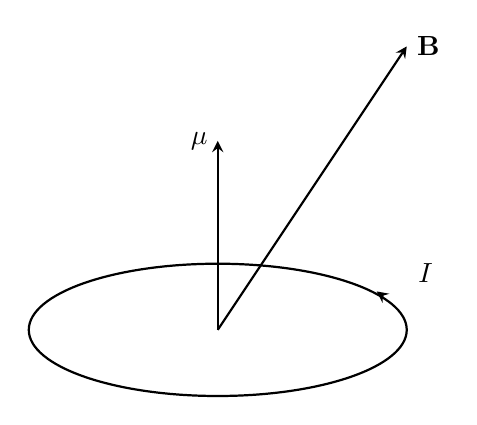
\begin{tikzpicture}[scale=1.2,>=stealth]

% --- Parte destra: Spira con corrente ---
\draw[thick] (6,0) ellipse (2cm and 0.7cm);

% Corrente I lungo ellisse (arco ellittico)
\draw[->,thick] (7.75,0.35) arc[start angle=20,end angle=25,x radius=2cm,y radius=0.7cm];
\node at (8.2,0.6) {$I$};

% Momento magnetico mu
\draw[->,thick] (6,0) -- (6,2) node[left] {$\mu$};

% Campo magnetico B
\draw[->,thick] (6,0) -- (8,3) node[right] {$\mathbf{B}$};

\end{tikzpicture}
}
\caption{Spira percorsa da corrente in un campo magnetico}
\label{fig:3_DipoloMag}
\end{figure}

Il momento magnetico dipolare è dato da:
\[
\vec{\mu} = I S\,\hat{\imath}_n
\]
dove $\hat{\imath}_n$ è la normale alla superficie $S$, orientata secondo la regola della mano destra rispetto alla corrente $I$.

Si consideri un tratto elementare \(d\vec{s}\) della spira; su di esso agisce la forza di Lorentz, poiché le cariche al suo interno sono messe in moto dalla corrente elettrica:
\[
d\vec{F} = I\,d\vec{s} \times \vec{B}
\]
Integrando su tutta la lunghezza della spira si ottiene:
\[
\vec{F} = \oint_{\partial S} I\,d\vec{s} \times \vec{B}
\]
Poiché la corrente e il campo \(\vec{B}\) sono costanti, possono essere portati fuori dal segno di integrale:
\[
\vec{F} = I\left( \oint_{\partial S} d\vec{s} \right) \times \vec{B}
\]
Siccome la spira è in equilibrio, la somma di tutti i contributi elementari è nulla; di conseguenza la forza risultante è nulla:
\[
\vec{F} = \vec{0}
\]
ovvero:
\[
I\left( \oint_{\partial S} d\vec{s} \right) \times \vec{B} = \vec{0}
 \Longleftrightarrow
\left( \oint_{\partial S} d\vec{s} \right) \times \vec{B} = \vec{0}
\]

Anche se la forza netta agente sulla spira è nulla, possono comunque esistere momenti torcenti. Poiché la forza agente sulla spira elementare è nulla, il momento delle forze risulta indipendente dal polo scelto. La coppia agente sull’elemento infinitesimo è data da:
\[
d\vec{N} = \vec{r} \times d\vec{F}
\]
La coppia, o momento torcente, può essere denotata anche con \(\vec{\tau}\). Integrando lungo la spira si ottiene:
\[
\vec{N} = \oint_{\partial S} \vec{r} \times d\vec{F}
\]
Sostituendo la forza di Lorentz \(d\vec{F} = I\,d\vec{s} \times \vec{B}\), si ha:
\[
\vec{N} = I \oint_{\partial S} \vec{r} \times (d\vec{s} \times \vec{B})
\]
Dati tre vettori, è valida l’identità:
\[
\vec{a} \times (\vec{b} \times \vec{c}) = (\vec{a}\cdot\vec{c})\,\vec{b} - (\vec{a}\cdot\vec{b})\,\vec{c}
\]
Applicando tale relazione, l'espressione del momento si scrive come:
\[
\vec{N} = I \oint_{\partial S} \big[(\vec{r}\cdot\vec{B})\,d\vec{s} - \vec{B}\,(\vec{r}\cdot d\vec{s})\big]
\]
Poiché il vettore \(\vec{r}\) appartiene alla spira, risulta \(d\vec{s} = d\vec{r}\), e dunque:
\[
\vec{N} = I \oint_{\partial S} \big[(\vec{r}\cdot\vec{B})\,d\vec{r} - \vec{B}\,(\vec{r}\cdot d\vec{r})\big]
\]
Il termine \(\vec{r}\cdot d\vec{r}\) può essere riscritto come:
\[
\vec{r}\cdot d\vec{r} = \dfrac{1}{2}\,d(\vec{r}\cdot\vec{r})
\]
per cui:

\[
\vec{N} = I\oint_{\partial S}{\left( \vec{r} \cdot \vec{B} \right)d\vec{r}} - I\oint_{\partial S}{\vec{B}\left( \vec{r} \cdot d\vec{r} \right)} = I\oint_{\partial S}{\left( \vec{r} \cdot \vec{B} \right)d\vec{r}} - \dfrac{1}{2}I\vec{B}\oint_{\partial S}{d\left( \vec{r} \cdot \vec{r} \right)}
\]

L'ultimo termine è l'integrale esteso a una linea chiusa di una forma differenziale esatta, dunque, è nullo:

\[
\oint_{\partial S}{d\left( \vec{r} \cdot \vec{r} \right)} = 0
\]

Pertanto, la coppia risulta:

\[
\vec{N} = I\oint_{\partial S}{\left( \vec{r} \cdot \vec{B} \right)d\vec{r}}
\]

Per risolvere tale integrale si considera la quantità \(d\left( \left( \vec{r} \cdot \vec{B} \right)\vec{r} \right)\); si applicano le proprietà del differenziale:

\[
d\left( \left( \vec{r} \cdot \vec{B} \right)\vec{r} \right) = \left( d\vec{r} \cdot \vec{B} \right)\vec{r} + \left( \vec{r} \cdot \vec{B} \right)d\vec{r} + \left( \vec{r} \cdot d\vec{B} \right)\vec{r}
\]

Dato che il campo è uniforme, \(d\vec{B} = 0\). Per cui:

\[
d\left( \left( \vec{r} \cdot \vec{B} \right)\vec{r} \right) = \left( d\vec{r} \cdot \vec{B} \right)\vec{r} + \left( \vec{r} \cdot \vec{B} \right)d\vec{r}
\]

Si ricava la quantità \(\left( \vec{r} \cdot \vec{B} \right)d\vec{r}\), presente nell'espressione della coppia:

\[
\left( \vec{r} \cdot \vec{B} \right)d\vec{r} = d\left( \left( \vec{r} \cdot \vec{B} \right)\vec{r} \right) - \left( d\vec{r} \cdot \vec{B} \right)\vec{r}
\]

Per applicare nuovamente la proprietà sul prodotto vettore di tre vettori, si aggiunge e sottrae \(\left( \vec{r} \cdot \vec{B} \right)d\vec{r}\) al secondo membro:

\[
\left( \vec{r} \cdot \vec{B} \right)d\vec{r} = d\left( \left( \vec{r} \cdot \vec{B} \right)\vec{r} \right) - \left( d\vec{r} \cdot \vec{B} \right)\vec{r} - \left( \vec{r} \cdot \vec{B} \right)d\vec{r} + \left( \vec{r} \cdot \vec{B} \right)d\vec{r}
\]

Dove:

\[
\left( \vec{r} \cdot \vec{B} \right)d\vec{r} - \left( d\vec{r} \cdot \vec{B} \right)\vec{r} = \vec{r} \times d\vec{r} \times \vec{B}
\]

Per cui si ha:

\[
\left( \vec{r} \cdot \vec{B} \right)d\vec{r} = d\left( \left( \vec{r} \cdot \vec{B} \right)\vec{r} \right) + \vec{r} \times d\vec{r} \times \vec{B} - \left( \vec{r} \cdot \vec{B} \right)d\vec{r} \Leftrightarrow 2\left( \vec{r} \cdot \vec{B} \right)d\vec{r} = d\left( \left( \vec{r} \cdot \vec{B} \right)\vec{r} \right) + \vec{r} \times d\vec{r} \times \vec{B}
\]

In definitiva, si ha:

\[
\left( \vec{r} \cdot \vec{B} \right)d\vec{r} = \dfrac{1}{2}d\left( \left( \vec{r} \cdot \vec{B} \right)\vec{r} \right) + \dfrac{1}{2}\vec{r} \times d\vec{r} \times \vec{B}
\]

Sostituendo tale risultato nell’espressione della coppia si ha::

\[
\vec{N} = I\oint_{\partial S}{\left( \vec{r} \cdot \vec{B} \right)d\vec{r}} = \dfrac{1}{2}\ I\oint_{\partial S}{d\left( \left( \vec{r} \cdot \vec{B} \right)\vec{r} \right)} + \dfrac{1}{2}\ I\oint_{\partial S}{\vec{r} \times d\vec{r} \times \vec{B}}
\]

Il primo termine è nullo, essendo una circuitazione di una forma differenziale esatta, quindi:

\[
\oint_{\partial S}{d\left( \left( \vec{r} \cdot \vec{B} \right)\vec{r} \right)} = \vec{0}
\]

Per cui si ha:

\[
\vec{N} = \dfrac{1}{2}\ I\oint_{\partial S}{\vec{r} \times d\vec{r} \times \vec{B}}
\]

Siccome il campo è costante lungo tutto il percorso di integrazione, può essere portato all'esterno del simbolo di integrale:

\[
\vec{N} = \dfrac{1}{2}\ I\left( \oint_{\partial S}{\vec{r} \times d\vec{r}} \right) \times \vec{B}
\]

Si definisce il \textbf{momento magnetico} della spira:

\[
\vec{\mu} = \dfrac{1}{2}\ I\oint_{\partial S}{\vec{r} \times d\vec{r}} = IS{\hat{\imath}}_{n}
\]

La coppia \(\vec{N}\) può, in definitiva, essere espressa come:

\[
\vec{N} = \vec{\mu} \times \vec{B}
\]

Nel caso più generale, il momento magnetico di una distribuzione continua di corrente in un volume \(V\) è dato da:

\[
\vec{\mu} = \dfrac{1}{2}\int_{V}{\vec{r} \times \vec{J}dV}
\]

\subsection{Momento magnetico di un anello rotante}\label{momento-magnetico-di-un-anello-rotante}

Si vuole calcolare il momento magnetico di un anello sottile di raggio \(R\), massa \(M\) e carica \(q\) distribuita uniformemente, che ruota con velocità angolare \(\omega\) attorno ad un asse ortogonale al piano in cui giace l'anello e passante per il centro.

\begin{figure}[ht]
\centering
\resizebox{0.196\textwidth}{!}{%
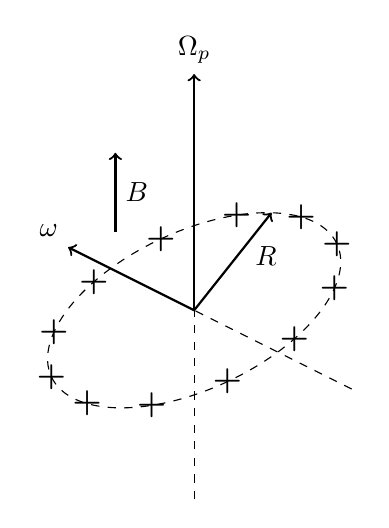
\begin{tikzpicture}[scale=2]

% Parametri ellisse
\def\a{1}   % semiasse maggiore
\def\b{0.5} % semiasse minore
\def\rot{25} % angolo di rotazione in gradi

% Ellisse inclinata corretta
\begin{scope}[rotate=\rot]
    \draw[dashed] (0,0) ellipse (1 and 0.5);
\end{scope}

% Cariche positive distribuite lungo ellisse inclinata
\foreach \angle in {0,30,...,345} {
    \pgfmathsetmacro{\x}{\a*cos(\angle)*cos(\rot) - \b*sin(\angle)*sin(\rot)}
    \pgfmathsetmacro{\y}{\a*cos(\angle)*sin(\rot) + \b*sin(\angle)*cos(\rot)}
    \node at (\x,\y) {\textbf{\large +}};
}

% Linea verticale tratteggiata (Omega_p)
\draw[dashed] (0,-1.2) -- (0,1.5);
\draw[->,thick] (0,0) -- (0,1.5) node[above] {$\Omega_p$};

% Freccia omega inclinata verso l'alto (effetto 3D)
\draw[->,thick] (0,0) -- (-0.8,0.4) node[above left] {$\omega$};
\draw[dashed] (1,-0.5) -- (0,0);

% Vettore B (verticale)
\draw[->,thick] (-0.5,0.5) -- (-0.5,1) node[midway,right] {$B$};

% Raggio R (dall'origine verso bordo ellisse)
\pgfmathsetmacro{\Rx}{\a*cos(45)*cos(\rot) - \b*sin(45)*sin(\rot)}
\pgfmathsetmacro{\Ry}{\a*cos(45)*sin(\rot) + \b*sin(45)*cos(\rot)}
\draw[->,thick] (0,0) -- (\Rx,\Ry) node[pos=0.3, above right, xshift=10pt, yshift=2pt] {$R$};

\end{tikzpicture}
}
\caption{Anello rotante nel campo magnetico}
\label{fig:3_RotRing}
\end{figure}

L’anello, ruotando, genera una corrente la cui intensità media è:

\[
I = \dfrac{q}{T}
\]

Dove \(T\) è il periodo dell'oscillazione dato da:

\[
T = \dfrac{2\pi}{\omega}
\]

Per cui la corrente è data da:

\[
I = \dfrac{q}{T} = q\dfrac{\omega}{2\pi}
\]

L'anello è assimilabile a una spira percorsa da corrente, dunque, il suo momento magnetico è dato da:

\[
\vec{\mu} = IS{\hat{\imath}}_{n} = q\dfrac{\omega}{2\pi}\pi R^{2}{\hat{\imath}}_{n}
\]

Semplificando, si ottiene il momento magnetico:

\[
\vec{\mu} = \dfrac{1}{2}q\omega R^{2}{\hat{\imath}}_{n}
\]

\subsection{Momento magnetico per un guscio sferico}\label{momento-magnetico-per-un-guscio-sferico}

Si vuole calcolare il momento magnetico di uno strato sferico sottile di raggio \(R\), massa \(M\) e carica \(Q\) distribuita uniformemente, che ruota con velocità angolare \(\omega\) attorno ad un asse passante per il centro della sfera.

\begin{figure}[ht]
\centering
\resizebox{0.59\textwidth}{!}{%
\begin{tikzpicture}[scale=2.5, >=stealth, line cap=round, line join=round]
    % Definizioni di base
    \def\R{1.6} % Raggio della sfera
    \def\thetaValue{60} % Angolo polare \vartheta in gradi
    
    % *** Parametri per l'effetto 3D (prospettiva) ***
    \def\yAxisScale{0.4} % Raggio y dell'ellisse per la profondità (0.4 è un buon compromesso)

    % Coordinate sferiche (in base a \thetaValue)
    \pgfmathsetmacro\r{\R*sin(\thetaValue)} % raggio dell'anello: R*sin(\vartheta)
    \pgfmathsetmacro\z{\R*cos(\thetaValue)} % coordinata z: R*cos(\vartheta)

    % --- Parametri per lo spessore infinitesimo (d\vartheta) ---
    \def\dTheta{3} % Metà della variazione d\vartheta per l'anello in gradi
    \pgfmathsetmacro\thetaUpper{\thetaValue - \dTheta} % Angolo superiore
    \pgfmathsetmacro\thetaLower{\thetaValue + \dTheta} % Angolo inferiore
    
    % Coordinate per i bordi dell'anello
    \pgfmathsetmacro\rUpper{\R*sin(\thetaUpper)}
    \pgfmathsetmacro\zUpper{\R*cos(\thetaUpper)}
    \pgfmathsetmacro\rLower{\R*sin(\thetaLower)}
    \pgfmathsetmacro\zLower{\R*cos(\thetaLower)}
    
    % --- Asse e Origine ---
    
    % Asse z (asse di rotazione)
    \draw[->, very thick] (0, 0, 0) -- (0, \R + 0.5, 0) node[above] {$z$};
    \draw[dashed, gray] (0, 0, 0) -- (0, -\R-0.1, 0);
        % Asse x 
    \draw[->, very thick] (0, 0, 0) -- (\R + 0.5, 0, 0) node[above] {$x$};
    \draw[dashed, gray] (0, 0, 0) -- (-\R-0.1, 0, 0);
        % Asse y
    \draw[->, very thick] (0, 0, 0) -- (0, 0, \R + 0.5) node[above] {$z$};
    \draw[dashed, gray] (0, 0, 0) -- (0, 0, -\R-0.1);

    % Centro della sfera (Origine O)
    \coordinate (O) at (0, 0);
    \draw[fill] (O) circle (1.5pt) node[below right] {$O$};

    % Linea per \omega (velocità angolare)
    \draw[->, very thick] (0.2, \R + 0.1) -- (0.2, \R + 0.4);
    \node[right] at (0.2, \R + 0.25) {$\vec{\omega}=\omega\,\hat{z}$};
    
    % --- Disegno della Sfera 3D (Simulata) ---

    % 1. Parte nascosta (posteriore) della sfera (sotto l'anello)
    \draw[thick, gray] (-\R, 0) arc (180:360:\R cm and \R*\yAxisScale cm); % Metà inferiore (nascosta)
    \draw[dashed, gray] (-\R, 0) arc (180:0:\R cm and \R*\yAxisScale cm); % Metà superiore (visibile)

    % 2. Contorno verticale (circonferenza)
    \draw[thick, gray] (0, 0) circle (\R);

    % --- Anello Elementare (Guscio) ---
    
    % L'anello è disegnato come due ellissi (bordo superiore e bordo inferiore)
    % e una superficie curva (riempimento) tra i due.
    
    % 1. Parte nascosta (posteriore) dell'anello
    \draw[dashed, blue!70!cyan] (0, \zUpper) ellipse (\rUpper cm and \rUpper*\yAxisScale cm); % Bordo superiore
    \draw[dashed, blue!70!cyan] (0, \zLower) ellipse (\rLower cm and \rLower*\yAxisScale cm); % Bordo inferiore

% ============================
%   1. SUPERFICIE (posteriore)
% ============================
\path[fill=blue!30, opacity=0.7]
  % Arco posteriore superiore
  (\rUpper, \zUpper)
    arc[start angle=0, end angle=180,
        x radius=\rUpper, y radius=\rUpper*\yAxisScale]
  --
  (-\rLower, \zLower)
  % Arco posteriore inferiore
    arc[start angle=180, end angle=0,
        x radius=\rLower, y radius=\rLower*\yAxisScale]
  -- cycle;


% ============================
%   3. BORDI ANTERIORI (visibili)
% ============================
\draw[line width=2pt, blue!70!cyan]
  (\rUpper, \zUpper)
    arc[start angle=0, end angle=-180,
        x radius=\rUpper, y radius=\rUpper*\yAxisScale];

\draw[line width=2pt, blue!70!cyan]
  (\rLower, \zLower)
    arc[start angle=0, end angle=-180,
        x radius=\rLower, y radius=\rLower*\yAxisScale];

\path[fill=blue!40, opacity=0.7]
  % Arco posteriore superiore
  (\rUpper, \zUpper)
    arc[start angle=0, end angle=-180,
        x radius=\rUpper, y radius=\rUpper*\yAxisScale]
  --
  (-\rLower, \zLower)
  % Arco posteriore inferiore
    arc[start angle=-180, end angle=0,
        x radius=\rLower, y radius=\rLower*\yAxisScale]
  -- cycle;
        
  % collegamento inferiore sinistra → destra
  --
  (\rLower, \zLower)
  % Arco anteriore inferiore (ritorno)
    arc[start angle=0, end angle=-180,
        x radius=\rLower, y radius=\rLower*\yAxisScale]
  -- cycle;
  
    % Linee di collegamento laterali (visibili)
    \draw[line width=2pt, blue!70!cyan] (\rUpper, \zUpper) -- (\rLower, \zLower);
    \draw[line width=2pt, blue!70!cyan] (-\rUpper, \zUpper) -- (-\rLower, \zLower);

    % --- Etichettatura dei parametri ---
    
    % Raggio 'r' dell'anello (al punto medio \z)
    \draw[<->, dashed, red] (0, \z) -- (\r, \z);
    \node[above] at (\r*0.5 + 0.5, \z + 0.1) {Raggio: $r=R\sin\vartheta$};
    
    % Raggio R della sfera (sul piano xz, passa attraverso il punto medio)
    \draw[->, very thick] (O) -- (\r, \z); 
    \node[right] at (\r*0.5 - 0.2, \z*0.5 + 0.1) {$R$};
    
    % Angolo \vartheta
    \draw[thick] (0.3, 0) arc (0:\thetaValue/2:0.3);
    \node[right] at (0.3, 0.1) {$\vartheta$};

    % Larghezza R d\vartheta (sulla superficie)
    
    % Coordinate per la freccia di larghezza (all'esterno della sfera)
    \coordinate (P_Top_Ext) at (\rUpper+0.1, \zUpper);
    \coordinate (P_Bottom_Ext) at (\rLower+0.1, \zLower);
    
    % Frecce per la larghezza R d\vartheta
    \draw[<->, very thick, red!70!black, shorten >= 1pt, shorten <= 1pt] 
        (P_Top_Ext) -- (P_Bottom_Ext);
    
    % Etichetta centrata sullo spessore
    \node[right, xshift=5pt] at ($(P_Top_Ext)!0.5!(P_Bottom_Ext)$) {Larghezza: $R\,d\vartheta$};

    % Elemento di area (etichette testuali)
    \node[below right, align=left, text=black!80!green, font=\small] at (\R + 0.05, -\R + 0.1) {
        \textbf{Elemento di area $dS$:}\\
        $\text{Circonf.} \times \text{Larghezza}$
    };
    \node[below right, align=left, text=black!80!green, font=\small] at (\R + 0.05, -\R + 0.5) {
        $dS = (2\pi r)(R\,d\vartheta)$\\
        $dS = 2\pi R^2\sin\vartheta\,d\vartheta$
    };
    
\end{tikzpicture}
}
\caption{Guscio sferico}
\label{fig:3_SferaCava}
\end{figure}

Si pone l'asse \(z\) coincidente con l'asse di rotazione, per cui \(\vec{\omega}=\omega\,\hat{z}\). Si suddivide la superficie sferica in anelli infinitesimi, ciascuno giacente su un piano ortogonale all'asse \(z\). In corrispondenza dell'angolo polare \(\vartheta\) l'anello ha:

\[
\text{raggio: } r=R\sin\vartheta,\qquad
\text{lunghezza: } 2\pi R\sin\vartheta,\qquad
\text{larghezza (sulla sfera): } R\,d\vartheta.
\]

L'elemento di area dell'anello è quindi:
\[
dS = (2\pi R\sin\vartheta)(R\,d\vartheta)=2\pi R^{2}\sin\vartheta\,d\vartheta.
\]

Se \(\sigma\) è la densità superficiale di carica uniforme, la carica dell'anello è \(dq=\sigma\,dS\) e la corrente associata alla sua rotazione è:
\[
dI=\dfrac{dq}{T}=\dfrac{\sigma\,dS}{T}=\dfrac{\omega\sigma}{2\pi}\,2\pi R^{2}\sin\vartheta\,d\vartheta
=\omega\sigma R^{2}\sin\vartheta\,d\vartheta,
\]
con \(T=2\pi/\omega\) periodo di rotazione della sfera. L'area della spira (anello) è \(S=\pi (R\sin\vartheta)^{2}\), dunque il momento magnetico elementare vale:
\[
d\vec{\mu}=S\,dI\,\hat{z}
= \pi R^{2}\sin^{2}\vartheta\;\omega\sigma R^{2}\sin\vartheta\,d\vartheta\;\hat{z}
= \pi\omega\sigma R^{4}\sin^{3}\vartheta\,d\vartheta\;\hat{z}.
\]

Per le ipotesi fatte sul sistema di riferimento, risulta che \({\hat{\imath}}_{n} = {\hat{\imath}}_{z}\). Infatti, il momento magnetico è diretto come \(\vec{\omega}\). Svolgendo i prodotti, si ha:

\[
d\vec{\mu} = \pi\omega\sigma R^{4}\sin^{3}\vartheta\ d\vartheta{\hat{\imath}}_{z}
\]

Il momento magnetico è ottenuto integrando l'equazione ottenuta su tutti i possibili valori assunti da \(\vartheta\), ovvero:

\[
\vec{\mu} = \int_{0}^{\pi}{\pi\omega\sigma R^{4}\sin^{3}\vartheta\ d\vartheta{\hat{\imath}}_{z}} = \pi\omega\sigma R^{4}\int_{0}^{\pi}{\sin^{3}\vartheta\ d\vartheta}{\hat{\imath}}_{z}
\]

Si risolve l'integrale. Per le relazioni trigonometriche è possibile scrivere:

\[
\int_{0}^{\pi}{\sin^{3}\vartheta d\vartheta} = \int_{0}^{\pi}{\left( \dfrac{3\sin\vartheta - \sin{3\vartheta}}{4} \right)d\vartheta} = \dfrac{1}{4}\left( 3\int_{0}^{\pi}{\sin\vartheta d\vartheta} - \int_{0}^{\pi}{\sin{3\vartheta}d\vartheta} \right)
\]

Dove:

\[
3\int_{0}^{\pi}{\sin\vartheta d\vartheta} = 3\left\lbrack - \cos\vartheta \right\rbrack_{0}^{\pi} = 3\left( - \cos\pi + \cos 0 \right) = 3(1 + 1) = 6
\]

\[
\int_{0}^{\pi}{\sin{3\vartheta}d\vartheta} = - \dfrac{1}{3}\left\lbrack \cos{3\vartheta} \right\rbrack_{0}^{\pi} = - \dfrac{1}{3}\left( \cos{3\pi} - \cos 0 \right) = - \dfrac{1}{3}( - 1 - 1) = \dfrac{2}{3}
\]

Nel complesso, l'integrale è dato da:

\[
\int_{0}^{\pi}{\sin^{3}\vartheta d\vartheta} = \dfrac{1}{4}\left( 6 - \dfrac{2}{3} \right) = \dfrac{1}{4}\left( \dfrac{18 - 2}{3} \right) = \dfrac{1}{4}\dfrac{16}{3} = \dfrac{4}{3}
\]

Il momento magnetico è dato da:

\[
\vec{\mu} = \dfrac{4}{3}\ \pi\omega\sigma R^{4}{\hat{\imath}}_{z}
\]

La superficie totale della sfera è data da:

\[
S = 4\pi R^{2}
\]

Il prodotto della densità superficiale di carica \(\sigma\) per la superficie \(S\) restituisce la carica globale \(Q\). Il momento magnetico può essere scritto come:

\[
\vec{\mu} = \dfrac{1}{3}\ \omega QR^{2}{\hat{\imath}}_{z}
\]

\subsection{Momento magnetico per una sfera}\label{momento-magnetico-per-una-sfera}

Si vuole calcolare il momento magnetico di una sfera raggio \(R\), massa \(M\) e carica \(Q\) distribuita uniformemente, che ruota con velocità angolare \(\omega\) attorno ad un asse passante per il centro della sfera.

\begin{figure}[ht]
\centering
%\resizebox{0.57\textwidth}{!}
\caption{Sfera rotante}
\label{fig:3_RotSphere}
\end{figure}

Si utilizzano le coordinate sferiche \(r\), \(\vartheta\), \(\varphi\). Si assume come polo il centro \(O\) della sfera carica e come asse polare il diametro parallelo alla velocità angolare \(\omega\). Risulta che:

\[
r \in \left[ 0; R\right],\ \vartheta \in \left[ 0;\pi\right],\ \varphi \in \left[ 0;2\pi\right]
\]

Si indica con \(\rho\) la densità di carica volumetrica. Il volumetto \(dV\) contiene una carica \(dq\):

\[
dq = \rho dV
\]

Un elemento di volume $dV$ contribuisce alla densità di corrente volumetrica $\vec{J}$, data da:

\[
\vec{J} = \rho \vec{v}
\]

Poiché la sfera ruota con velocità angolare \(\vec{\omega}\) e la carica ha densità \(\rho\), la densità di corrente volumetrica è:

\[
\vec{J} = \rho \vec{v} = \rho \left( \vec{\omega} \times \vec{r}\right)
\]

per calcolare il momento magnetico di un corpo di volume \(V\) con densità di corrente \(J\), si usa la formula generale:

\[
\vec{\mu} = \dfrac{1}{2}\int_{V}{\vec{r} \times \vec{J}dV}
\]

Sostituendo la densità di corrente dell'elemento di volume infinitesimo nella definizione del momento magnetico si ha:

\[
\vec{\mu} = \dfrac{1}{2}\int_{V}{\vec{r} \times \left(\rho \left( \vec{\omega} \times \vec{r}\right)\right)dV}
\]

Nell'ipotesi di densità di carica costante in tutto il volume, è possibile portare all'esterno del simbolo di integrale \(\rho\):

\[
\vec{\mu} = \dfrac{1}{2}\rho\int_{V}{\vec{r} \times \left( \vec{\omega} \times \vec{r}\right)dV}
\]

Si considera il triplo prodotto vettoriale all'interno dell'integrale e si utilizza l'identità nota:

\[
\vec{a} \times (\vec{b} \times \vec{c}) = (\vec{a} \cdot \vec{c})\vec{b} - (\vec{a} \cdot \vec{b})\vec{c}
\]

Ponendo \(\vec{a} = \vec{r}\), \(\vec{b} = \vec{\omega}\), e \(\vec{c} = \vec{r}\), l'espressione \(\vec{r} \times \vec{\omega} \times \vec{r} \) diventa:

\[
\vec{r} \times \vec{\omega} \times \vec{r} = (\vec{r} \cdot \vec{r})\vec{\omega} - (\vec{r} \cdot \vec{\omega})\vec{r}
\]

Ricordando che \(\vec{r} \cdot \vec{r} = r^2\), l'ultima relazione può essere scritta come:

\[
\vec{r} \times \vec{\omega} \times \vec{r} = r^{2}\vec{\omega}-\left(\vec{r}\cdot\vec{\omega}\right)\vec{r}
\]

Per ipotesi, la rotazione avviene lungo la direzione \(\hat{\imath}_{z}\), per cui \(\vec{\omega}=\omega \hat{\imath}_{z}\). Inoltre, è possibile esprimere il vettore posizione in coordinate sferiche:

\[
\vec{r} = r (\sin\vartheta \cos\varphi\,\hat{\imath}_x + \sin\vartheta \sin\varphi\,\hat{\imath}_y + \cos\vartheta\,\hat{\imath}_z)
\]

Il prodotto scalare tra il vettore posizione e la velocità angolare avviene solamente tre le componenti lungo \(\hat{\imath}_z\):

\[
\vec{r}\cdot \vec{\omega} = r (\sin\vartheta \cos\varphi\,\hat{\imath}_x + \sin\vartheta \sin\varphi\,\hat{\imath}_y + \cos\vartheta\,\hat{\imath}_z) \cdot \omega\hat{\imath}_z = r\omega\cos\vartheta\
\]

Il prodotto vettoriale triplo si scrive come:

\[
\vec{r} \times \vec{\omega} \times \vec{r} = {r}^2\omega\hat{\imath}_z - \left(\omega r \cos\vartheta\right)\left(r (\sin\vartheta \cos\varphi\,\hat{\imath}_x + \sin\vartheta \sin\varphi\,\hat{\imath}_y + \cos\vartheta\,\hat{\imath}_z)\right)
\]

Svolgendo i prodotti, si ricava:

\[
\vec{r} \times \vec{\omega} \times \vec{r} = {r}^2\omega\hat{\imath}_z - r^{2}\omega\left( \sin{\vartheta}\cos{\varphi}\,\cos\vartheta\hat{\imath}_{x} + \sin\vartheta \sin\varphi\,\cos\vartheta\hat{\imath}_y+\cos^2\vartheta\hat{\imath}_z\right)
\]

Sostituendo questo risultato nell'espressione vettoriale per il momento magnetico, si ottiene:

\[
\vec{\mu} = \dfrac{1}{2}\rho\int_{V}{ \left({r}^2\omega\hat{\imath}_z - r^{2}\omega\left( \sin{\vartheta}\cos{\varphi}\,\cos\vartheta\hat{\imath}_{x} + \sin\vartheta \sin\varphi\,\cos\vartheta\hat{\imath}_y+\cos^2\vartheta\hat{\imath}_z\right)\right)dV}
\]

Si raccoglie \(\omega\) che, essendo costante rispetto la posizione, può essere portata fuori dal simbolo di integrale:

\[
\vec{\mu} = \dfrac{1}{2}\rho\omega \int_{V}{ \left({(r}^2\hat{\imath}_z - r^{2}\left( \sin{\vartheta}\cos{\varphi}\,\cos\vartheta\hat{\imath}_{x} + \sin\vartheta \sin\varphi\,\cos\vartheta\hat{\imath}_y+\cos^2\vartheta\hat{\imath}_z\right)\right)dV}
\]

Si divide l'integrale in base alle componenti spaziali delle coordinate sferiche:

\[
\vec{\mu} = \dfrac{1}{2}\rho\omega \left(\int_{V}{ \left(r^2\,\hat{\imath}_z - r\cos^{2}{\vartheta} \right)\hat{\imath}_z\,dV} - \int_{V}{\left( r^{2} \sin{\vartheta}\cos{\varphi}\,\cos\vartheta\hat{\imath}_{x} \right) \,dV} - \int_{V}{\left( r^2sin\vartheta \sin\varphi\,\cos\vartheta\hat{\imath}_y\right) \,dV}\right)
\]

In coordinate sferiche, l'elemento di volume infinitesimo è il prodotto delle tre lunghezze elementari:

\[
dV = 
\underbrace{dr}_{\text{spessore radiale}}\,
\underbrace{(r\,d\vartheta)}_{\text{altezza meridiana}}\,
\underbrace{(r\sin\vartheta\,d\varphi)}_{\text{lunghezza azimutale}}
= r^{2}\sin\vartheta\,dr\,d\vartheta\,d\varphi
\]

Si risolve l'integrale contenente la componente lungo la direzione \(\hat{\imath}_x\). Utilizzando le coordinate sferiche e integrando su tutto il volume, si ottiene:

\[
\int_{V}{\left( r^{2} \sin{\vartheta}\cos{\varphi}\,\cos\vartheta \right) \,dV}=\int_{0}^{R}{\int_{0}^{\pi}{\int_{0}^{2\pi}{r^{2} \sin{\vartheta}\cos{\varphi}\,\cos\vartheta \left(r^{2}\sin\vartheta\right)d\varphi}d\vartheta}dr}=
\]

Per la linearità dell'operatore integrale è possibile scrivere:

\[
=\int_{0}^{R}{r^{4}\int_{0}^{\pi}{\sin^{2}{\vartheta}\cos{\vartheta}\int_{0}^{2\pi}{cos{\varphi}\,d\varphi}d\vartheta}dr}
\]

Nella relazione individuata il \(cos{\varphi}\) è integrato sul suo periodo, pertanto il suo risultato è nullo. Di conseguenza anche l'integrale complessivo è nullo:

\[
\int_{V}{\left( r^{2} \sin{\vartheta}\cos{\varphi}\,\cos\vartheta \right) \,dV}=\int_{0}^{R}{r^{4}\int_{0}^{\pi}{\sin^{2}\cos{\vartheta}\int_{0}^{2\pi}{cos{\varphi}\,d\varphi}d\vartheta}dr}=0
\]

Per l'integrazione lungo la componente \(\hat{\imath}_y\) vale un discorso analogo, dunque, anche questo contributo è nullo. Le componenti $\mu_x$ e $\mu_y$ del momento magnetico si annullano a causa della simmetria di rotazione della sfera attorno all'asse $\hat{\imath}_{z}$, espressa matematicamente dall'integrazione su $\varphi$ (l'angolo azimutale) che annulla i termini $\cos\varphi$ e $\sin\varphi$. Il momento magnetico totale è quindi solo in direzione $\hat{\imath}_z$:

\[
\vec{\mu} = \mu_z\,\hat{\imath}_z
\]

Al fine di valutare l'espressione del momento magnetico, bisogna risolvere l'integrale lungo l'asse di rotazione:

\[
\mu_{z} = \dfrac{1}{2}\rho\omega\int_{V}{\left(r^{2} - r^{2}\cos^2{\vartheta} \right) dV} = \dfrac{1}{2}\rho\omega\int_{V}{r^{2}\left(1 -\cos^2{\vartheta} \right) dV}
\]

Si utilizza l'identità trigonometrica \(1 - \cos^2{\vartheta} = \sin^2{\vartheta}\) e si sostituisce l'espressione del volumetto elementare \(dV = r^{2}\sin\vartheta drd\vartheta d\varphi\):

\[
\mu_{z} = \dfrac{1}{2}\rho\omega\int_{V}{r^{2}\sin^2{\vartheta} dV}=\dfrac{1}{2}\rho\omega\int_{0}^{R}{\int_{0}^{\pi}{\int_{0}^{2\pi}{r^{2}\sin^2{\vartheta} \left(r^{2}\sin\vartheta drd\vartheta d\varphi\right)}}}
\]

Riorganizzando i termini e separando gli integrali, si ricava:

\[
\mu_{z} = \dfrac{1}{2}\rho\omega \left(\int_{0}^{2\pi} d\varphi\right) \left(\int_{0}^{\pi} \sin^3{\vartheta} d\vartheta\right) \left(\int_{0}^{R} r^{4} dr\right)
\]

L'integrale sulla coordinata azimutale è:

\[
\int_{0}^{2\pi} d\varphi = 2\pi
\]

L'integrale sul raggio, è invece dato da:

\[
\int_{0}^{R} r^{4} dr = \left[ \dfrac{r^{5}}{5} \right]_{0}^{R} = \dfrac{R^{5}}{5}
\]

L'integrale sulla coordinata polare è:

\[
\int_{0}^{\pi}{\sin^{3}\vartheta d\vartheta} = \int_{0}^{\pi}{\left( \dfrac{3\sin\vartheta - \sin{3\vartheta}}{4} \right)d\vartheta} = \dfrac{1}{4}\left( 3\int_{0}^{\pi}{\sin\vartheta d\vartheta} - \int_{0}^{\pi}{\sin{3\vartheta}d\vartheta} \right)
\]

\[
\int_{0}^{\pi}{\sin^{3}\vartheta d\vartheta} = \int_{0}^{\pi}{\left( \dfrac{3\sin\vartheta - \sin{3\vartheta}}{4} \right)d\vartheta} = \dfrac{1}{4}\left( 3\int_{0}^{\pi}{\sin\vartheta d\vartheta} - \int_{0}^{\pi}{\sin{3\vartheta}d\vartheta} \right)
\]

Dove:

\[
3\int_{0}^{\pi}{\sin\vartheta d\vartheta} = 3\left\lbrack - \cos\vartheta \right\rbrack_{0}^{\pi} = 3\left( - \cos\pi + \cos 0 \right) = 3(1 + 1) = 6
\]

\[
\int_{0}^{\pi}{\sin{3\vartheta}d\vartheta} = - \dfrac{1}{3}\left\lbrack \cos{3\vartheta} \right\rbrack_{0}^{\pi} = - \dfrac{1}{3}\left( \cos{3\pi} - \cos 0 \right) = - \dfrac{1}{3}( - 1 - 1) = \dfrac{2}{3}
\]

Nel complesso, l'integrale è dato da:

\[
\int_{0}^{\pi} \sin^3{\vartheta} d\vartheta = \dfrac{4}{3}
\]

Di conseguenza, il momento magnetico della sfera è dato da:

\[
\mu_{z} = \dfrac{1}{2}\rho\omega \left( 2\pi \right) \left( \dfrac{4}{3} \right) \left( \dfrac{R^{5}}{5} \right) = \dfrac{4\pi}{15}\rho\omega R^5
\]

La carica totale \(Q\) è data dal prodotto della densità volumetrica \(\rho\) per il volume della sfera \(V=4\pi R^{3}/3\):

\[
Q=\rho V\Leftrightarrow \rho = \dfrac{Q}{V}
\]

Sostituendo il volume della sfera, si ottiene:

\[
Q=\rho V\Leftrightarrow \rho = \dfrac{Q}{V}=\dfrac{Q}{\dfrac{4}{3}\pi R^3}=\dfrac{3Q}{4\pi R^3}
\]

Sostituendo l'espressione di \(\rho\) nell'espressione per il momento magnetico lungo l'asse di rotazione, si ottiene:

\[
\mu_{z} = \dfrac{4\pi}{15}\omega R^5 \left( \dfrac{3Q}{4\pi R^3} \right)
\]

Semplificando:

\[
\mu_{z} = \dfrac{1}{5} Q \omega R^2
\]

Dato che il momento magnetico della sfera rotante è diretto lungo l'asse di rotazione, si ha:

\[
\vec{\mu} = \dfrac{1}{5} Q \omega R^{2}\hat{\imath}_z
\]

\section{Forza su piccola spira in un campo disomogeneo}\label{forza-su-piccola-spira-in-un-campo-disomogeneo}

La forza che agisce su una piccola spira percorsa da corrente, assimilabile a un \textbf{dipolo magnetico} $\vec{\mu}$, immersa in un campo di induzione magnetica $\vec{B}$ \textbf{non uniforme} è determinata dalla variazione spaziale dell'energia potenziale $U = - \vec{\mu} \cdot \vec{B}$.

La forza è data da $\vec{F} = -\vec{\nabla}U$:
\[
\vec{F} = -\vec{\nabla}\left( - \vec{\mu} \cdot \vec{B} \right) = \vec{\nabla}\left( \vec{\mu} \cdot \vec{B} \right)
\]

Poiché il momento magnetico $\vec{\mu}$ di una spira elementare è costante rispetto alla posizione $\vec{r}$, l'espressione $\vec{\nabla}(\vec{\mu} \cdot \vec{B})$ può essere semplificata utilizzando l'identità vettoriale generale:

\[
(\vec{\mu} \cdot \vec{\nabla}) = \mu_x\dfrac{\partial}{\partial x} + \mu_y\dfrac{\partial}{\partial y} + \mu_z\dfrac{\partial}{\partial z}
\]

L'espressione per la forza si riduce a:

\[
\vec{F} = \left(\vec{\mu} \cdot \vec{\nabla}\right) \vec{B}
\]

L'equazione, scritta in forma estesa, è:

\[
\begin{pmatrix}
F_{x} \\
F_{y} \\
F_{z}
\end{pmatrix} = \begin{pmatrix}
     \mu_x\dfrac{\partial}{\partial x} + \mu_y\dfrac{\partial}{\partial y} + \mu_z\dfrac{\partial}{\partial z}
\end{pmatrix}\begin{pmatrix}
B_{x} \\
B_{y} \\
B_{z}
\end{pmatrix} = \begin{pmatrix}
 \mu_x\dfrac{\partial B_x}{\partial x} + \mu_y\dfrac{\partial B_x}{\partial y} + \mu_z\dfrac{\partial B_x}{\partial z} \\
 \mu_x\dfrac{\partial B_y}{\partial x} + \mu_y\dfrac{\partial B_y}{\partial y} + \mu_z\dfrac{\partial B_y}{\partial z} \\
 \mu_x\dfrac{\partial B_z}{\partial x} + \mu_y\dfrac{\partial B_z}{\partial y} + \mu_z\dfrac{\partial B_z}{\partial z}
\end{pmatrix}
\]

Si suppone che il campo sia diretto solamente lungo \(z\), direzione lungo cui è variabile. In altre parole, il campo è $\vec{B} = B_{z}\left(z\right){\hat{\imath}}_{z}$. La forza, in questo contesto, può essere espressa come:
\[
\begin{pmatrix}
F_{x} \\
F_{y} \\
F_{z}
\end{pmatrix} = \begin{pmatrix}
      \mu_x\dfrac{\partial}{\partial x} + \mu_y\dfrac{\partial}{\partial y} + \mu_z\dfrac{\partial}{\partial z}
\end{pmatrix}\begin{pmatrix}
0 \\
0 \\
B_{z}\left(z\right)
\end{pmatrix} = \begin{pmatrix}
0 \\
0 \\
 \mu_z\dfrac{\partial B_z}{\partial z}
\end{pmatrix}
\]

La componente non nulla della forza è solamente quella lungo \(z\), data da:

\[F_{z} = \mu_{z}\dfrac{\partial B_{z}}{\partial z}\]

La forza $F_z$ dipende dalla \textbf{proiezione del momento magnetico} $\mu_{z}$ lungo la direzione del gradiente e dalla \textbf{pendenza} ($\partial B_{z}/\partial z$) del campo. Se $\mu_z$ e $\partial B_z / \partial z$ hanno lo stesso segno, la forza spinge la spira verso le regioni di campo più intenso.

Questa relazione è il principio fisico alla base dell'esperimento di \textbf{Stern-Gerlach}, dove un fascio di atomi (dipoli magnetici) viene deviato in un campo magnetico non uniforme.

\subsection{Esperimento di Stern-Gerlach}\label{esperimento-di-stern-gerlach}

L'esperimento di Stern-Gerlach (1922) fornisce la prova sperimentale della \textbf{quantizzazione spaziale} del momento magnetico dell'atomo.

Nel modello classico l'elettrone era visto come un pianeta orbitante intorno al nucleo, dunque, caratterizzato da un momento angolare dato dalla rivoluzione dell'elettrone intorno al nucleo e intorno al proprio asse.

\begin{figure}[ht]
\centering
\resizebox{0.41\textwidth}{!}{%
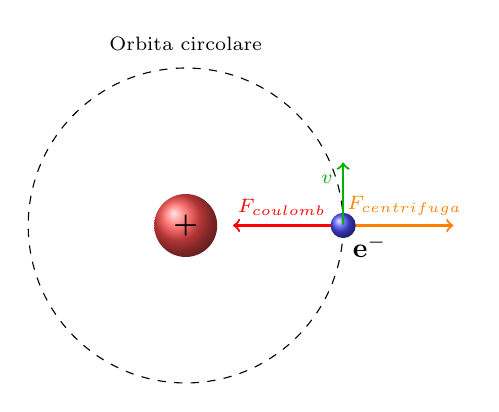
\begin{tikzpicture}[scale=2]
    % Nucleo
    \shade[ball color=red!70] (0,0) circle (0.2);
    \node at (0,0) {\textbf{+}}; % carica positiva
    
    % Orbita
    \draw[thin, dashed] (0,0) circle (1.0);
    \node[above] at (0,1.05) {\scriptsize Orbita circolare};
    
    % Elettrone
    \shade[ball color=blue!70] (1.0,0) circle (0.08);
    \node[below right] at (1.0,0) {\textbf{e$^-$}};
    
    % Forza coulombiana (verso il nucleo)
    \draw[->, thick, red] (0.92,0) -- (0.3,0)
        node[midway, above] {\scriptsize $F_{\text{coulomb}}$};
    
    % Forza centrifuga (verso l'esterno)
    \draw[->, thick, orange] (1.08,0) -- (1.7,0)
        node[midway, above] {\scriptsize $F_{\text{centrifuga}}$};
    
    % Velocità tangenziale
    \draw[->, thick, green!70!black] (1.0,0) -- (1.0,0.4)
        node[midway, above left] {\scriptsize $v$};
\end{tikzpicture}

}
\caption{Modello pl3netario dell'atomo}
\label{fig:3_ModPlan}
\end{figure}

È noto, inoltre, che la massa del nucleo è di molti ordini di grandezza maggiore rispetto quella dell'elettrone; dunque, è possibile ritenere il nucleo fermo rispetto all'elettrone.

Nel modello classico, l'elettrone orbita attorno al nucleo (considerato fermo, $m_{nucleo} \gg m_{e}$) con raggio $r$ e velocità $v$. L'elettrone, avendo carica $e$, genera una corrente $I$:

\[
I = \dfrac{{\Delta}q}{{\Delta}t}
\]

Dove, la carica coincide con quella dell'elettrone, mentre \({\Delta}t\) coincide con il periodo di rivoluzione della particella carica:

\[
I = \dfrac{{\Delta}q}{{\Delta}t} = \dfrac{e}{2\pi\dfrac{r}{v}} = \dfrac{ev}{2\pi r}
\]

Data la piccola corrente generata, esiste un momento magnetico \(\vec{\mu}\) ortogonale al piano sul quale l'elettrone esegue la sua orbita, con verso diretto in modo da vedere la corrente ruotare in senso antiorario. Per convenzione sulla corrente, l'elettrone deve ruotare in senso orario.

Il momento magnetico è dato da:

\[
\vec{\mu} = IS{\hat{\imath}}_{n}
\]

Si considera il modulo, si sostituisce l'espressione della corrente prodotta dall'elettrone e la superficie della spira descritta :

\[
\mu = IS = - \dfrac{ev}{2\pi r}\pi r^{2} = - \dfrac{evr}{2}
\]

Dove il segno meno è dovuto alla convenzione sulle correnti.

Sull'elettrone agisce un momento angolare \(\vec{L}\), dovuto all'orbita circolare descritto dall'elettrone, anch'esso ortogonale al piano dell'orbita, dato da:

\[
\vec{L} = m\vec{r} \times \vec{v}
\]

Si considera il modulo del momento angolare:

\[
L = mrv
\]

Si moltiplicano ambo i membri per \(e/2\):

\[
\dfrac{e}{2}L = \dfrac{e}{2}mrv
\]

Sostituendo l'espressione del momento magnetico, si ha:

\[
\dfrac{e}{2}L = m\mu
\]

Ricavano il momento magnetico in funzione del momento angolare, si ha:

\[
\mu = \dfrac{e}{2m}L
\]

In generale, se la particella ha carica \(q\) negativa, risulta:

\[
\vec{\mu} = - \dfrac{q}{2m}\vec{L}
\]

Dove \(\vec{\mu}\) è opposto a \(\vec{L}\) per la convenzione sulle correnti.

Sebbene l'ultima equazione sia stata ricavata nell'ambito della fisica classica, è valida anche in meccanica quantistica, in cui il punto di vista è completamente diverso.

I risultati dell'esperimento sono usati ancora oggi per dimostrare lo spin. Al tempo l'obiettivo era dimostrare l'esistenza del momento magnetico intrinseco e la sua quantizzazione spaziale. I due fisici eseguirono l'esperimento sugli atomi di \textbf{argento}, emessi da una sorgente. Questi atomi venivano deflessi da un campo magnetico non omogeneo, variabile lungo \(z\). 

L'argento è stato scelto proprio perché il suo momento angolare totale, derivante dagli elettroni di valenza, è dovuto essenzialmente a un singolo elettrone $s$-orbitale, semplificando l'interpretazione dei risultati.

La meccanica classica prevede che momento magnetico degli atomi di argento sia distribuito statisticamente in tutte le direzioni. Sugli atomi di argento agisce una forza data da:

\[
F_{i} = {\mu_{i}}_{z}\dfrac{\partial B_{z}}{\partial z}
\]

Dunque, ogni atomo subisce una deflessione dovuta alla proiezione del suo momento magnetico lungo l'asse \(z\) e dal gradiente del campo magnetico lungo lo stesso asse.

Nella teoria classica, dato che ogni atomo possiede un momento magnetico orientato casualmente, Stern e Gerlach si aspettavano di ottenere una linea retta compresa tra un massimo e minimo. Tutte le posizioni compresi tra questi due valori hanno tutti la stessa probabilità.

Tuttavia, i due scienziati rilevarono solo due punti di arrivo. I due dedussero che gli orientamenti dei momenti magnetici degli atomi non disposti in modo casuale ma in maniera quantizzata.

Questo risultato non può essere previsto dalla meccanica classica, ma viene spiegato dalla meccanica quantistica.

\begin{figure}[ht]
\centering
\resizebox{0.57\textwidth}{!}{%
\begin{tikzpicture}[>=Stealth, font=\sffamily]

% Traiettorie
\draw[thick] (-4,0) .. controls (-1,0.5) and (1,1) .. (4,2);
\draw[thick] (-4,0) .. controls (-1,-0.5) and (1,-1) .. (4,-2);

% Sorgente atomi
\draw[red, thick] (-4,0) circle (0.15cm);
\node[red, left] at (-2.5,-0.45) {sorgente atomi};

% Schermo rivelatore
\draw[red, thick] (4,2) circle (0.15cm);
\draw[red, thick] (4,-2) circle (0.15cm);
\draw[red, dotted, thick] (4,-2.5) -- (4,2.5);
\node[red, right] at (4,0) {schermo rivelatore};

% Freccia verticale con etichetta
\draw[->, thick] (0,-0.3) -- (0,2.5);
\node[above] at (0,2.5) {$\dfrac{\partial B_z}{\partial z}$};

\end{tikzpicture}
}
\label{fig:3_SternGerlach}
\caption{Esperimento di Stern-Gerlach}
\end{figure}

Il risultato non può essere spiegato dalla quantizzazione del momento angolare orbitale prevista da Bohr, ma dalla scoperta successiva del \textbf{momento angolare di spin} intrinseco ($\vec{S}$) dell'elettrone.
Per l'elettrone, il momento angolare di spin è quantizzato e può avere solo due proiezioni lungo l'asse $z$: $m_s = \pm 1/2$. Il momento magnetico di spin è legato a $\vec{S}$ da:
   
\[
\vec{\mu}_S = - g_e \dfrac{e}{2m_e}\vec{S} \quad \text{con } g_e \approx 2
\]

Dove $g_e$ è il fattore $g$ di Landé per lo spin.

Il risultato a due punti dello Stern-Gerlach è, di fatto, la prova diretta che l'elettrone possiede una proprietà quantistica intrinseca chiamata \textbf{spin}, che può essere orientata solo in due direzioni discrete ($\uparrow$ o $\downarrow$) rispetto a un asse di riferimento esterno.

La quantità fondamentale del magnetismo quantistico è il \textbf{Magnetone di Bohr}:

\[
\mu_B = \dfrac{e\hbar}{2m_e} \approx 9.27 \times 10^{-24} \text{ J/T}
\]
La forza magnetica misurata è quindi direttamente proporzionale a $\pm \mu_B$.

\subsection{Concetto di spin}\label{concetto-di-spin}

Il concetto di spin è inglobato nella meccanica quantistica e può essere visualizzato come la rotazione dell'elettrone intorno al suo asse. Lo spin determina un momento angolare e un momento magnetico. I due parametri sono antiparalleli e legati dal rapporto giromagnetico ($\gamma$).

\[\vec{\mu} = - \dfrac{q}{2m}\vec{L} = - \gamma_{e}\vec{L}\]

Il concetto di elettrone rotante non può essere considerato valido poiché, nel contesto della meccanica quantistica, l'elettrone è privo di estensione superficiale. Lo spin è una proprietà intrinseca della particella, non legata a rotazione spaziale.

In meccanica quantistica, ogni particella elementare o composta che possieda un momento angolare intrinseco (spin $\vec{S}$) o orbitale ($\vec{L}$) è associata a un momento magnetico $\vec{\mu}$. Il momento magnetico intrinseco ($\vec{\mu}_s$) di una particella è sempre proporzionale al suo spin ($\vec{S}$):

\[
\vec{\mu}_s = g \dfrac{q}{2m} \vec{S}
\]
Dove:
\begin{itemize}
    \item $q$ e $m$ sono, rispettivamente, la carica e la massa della particella (ad esempio, elettrone, protone, muone, ecc.);
    \item $\vec{S}$ è il momento angolare di spin della particella;
     \item $g$ è il \textbf{fattore giromagnetico} ($g$-factor) o \textbf{fattore di Landé}, un numero adimensionale che quantifica lo scostamento del momento magnetico dal valore atteso classico ($q/2m$).
\end{itemize}

Per l'elettrone, la formula è:
\[
\vec{\mu}_{e} = - g_{e} \dfrac{e}{2m_{e}} \vec{S}
\]

Il fattore $e/2m_{e}$ è l'unità naturale del magnetismo per l'elettrone ed è chiamato \textbf{Magnetone di Bohr} ($\mu_B$). Il fattore $g_e$ per l'elettrone libero è $g_e \approx 2.0023$ (la piccola deviazione da $g=2$ è spiegata dall'Elettrodinamica Quantistica, QED).

Per i nucleoni e nuclei, si usa la massa del protone ($m_p$) come riferimento per l'unità magnetica, poiché i momenti magnetici nucleari sono molto più piccoli:

\[
\vec{\mu}_{N} = g_{N} \dfrac{e}{2m_{p}} \vec{I}
\]
Dove:
\begin{itemize}
    \item \(e/2m_{p}\) è il magnetone nucleare ($\mu_N$);
    \item $\vec{I}$ è il momento angolare di spin nucleare;
    \item $g_N$ è il fattore $g$ nucleare, che è caratteristico di ciascun nucleo.
\end{itemize}

Per i nucleoni (protoni e neutroni) e i nuclei, i momenti magnetici sono significativamente più piccoli. Si usa il \textbf{Magnetone Nucleare} ($\mu_N$), basato sulla massa del protone ($m_p$):

\[
\mu_N = \dfrac{e\hbar}{2m_{p}} \ll \mu_B
\]

La relazione è data da:
\[
\vec{\mu}_{N} = g_{N} \dfrac{e}{2m_{p}} \vec{I}
\]

dove $\vec{I}$ è il momento angolare di spin nucleare e $g_N$ è il fattore $g$ nucleare, che non ha un valore universale come l'elettrone, ma è caratteristico di ciascun nucleo o nucleone.
Per un atomo in uno stato quantico definito, il momento magnetico totale ($\vec{\mu}_{tot}$) è proporzionale al momento angolare totale ($\vec{J} = \vec{L} + \vec{S}$):

\[
\vec{\mu}_{tot} = - g \dfrac{e}{2m_{e}} \vec{J}
\]
In questo caso, $g_J$ è il \textbf{fattore di Landé} per l'atomo intero, il cui valore dipende da come si accoppiano $\vec{L}$ e $\vec{S}$ (ad esempio, tramite l'accoppiamento $LS$).

In sintesi, la relazione $\vec{\mu} = g q/2m \vec{S}$ è la formula unificatrice in meccanica quantistica, con il fattore $g$ che incorpora la natura specifica della particella o del sistema considerato.

\section{Campo magnetico prodotto da un momento magnetico}\label{campo-magnetico-prodotto-da-un-momento-magnetico}
Si vuole determinare il campo $\vec{B}$ creato da un momento magnetico $\vec{\mu}$ di una piccola spira percorsa da corrente, a grandi distanze $R$. A tale scopo si considerano le equazioni di Maxwell per il campo induzione magnetica nel vuoto:

\[
\begin{cases}
\vec{\nabla} \cdot \vec{B} = 0 \\
\vec{\nabla} \times \vec{B} = \mu_{0}\left( \vec{J} + \varepsilon_{0}\dfrac{\partial\vec{E}}{\partial t} \right)
\end{cases}
\]

Se la lunghezza d'onda del campo incidente \(\lambda\) è molto maggiore della dimensione lineare dell'oggetto, è possibile ritenere il campo elettromagnetico lentamente variabile sulla superficie della spira, dunque:

\[
\dfrac{\partial\vec{E}}{\partial t} \simeq 0
\]

È possibile scrivere:

\[
\begin{cases}
\vec{\nabla} \cdot \vec{B} = 0 \\
\vec{\nabla} \times \vec{B} = \mu_{0}\vec{J}
\end{cases}
\]

Siccome il campo induzione magnetica è solenoidale, è possibile definire un \textbf{potenziale vettore}, tale che:

\[
\vec{B} = \vec{\nabla} \times \vec{A}
\]

Si sostituisce la definizione del potenziale vettore nella seconda equazione:

\[
\vec{\nabla} \times \vec{B} = \mu_{0}\vec{J} \Leftrightarrow \vec{\nabla} \times \vec{\nabla} \times \vec{A}
\]

Il rotore del rotore può essere scritto come:

\[
\vec{\nabla} \times \vec{\nabla} \times = \vec{\nabla}\left( \vec{\nabla} \cdot \  \right) - \nabla^{2}
\]

Dunque, si ottiene:

\[
\vec{\nabla}\left( \vec{\nabla} \cdot \vec{A} \right) - \nabla^{2}\vec{A} = \mu_{0}\vec{J}
\]

Il potenziale vettore non è univocamente definito, dunque, è possibile imporre la condizione, detta \textbf{gauge di Coulomb}:

\[
\vec{\nabla} \cdot \vec{A} = 0
\]

Si ottiene che il laplaciano del campo vettore è dato da:

\[
\nabla^{2}\vec{A} = - \mu_{0}\vec{J}
\]

Si dimostra che la soluzione è del tipo:

\[
\vec{A} = \dfrac{\mu_{0}}{4\pi}\int_{V}\dfrac{\vec{J}\left( {\vec{r}}' \right)}{\left| \vec{r} - {\vec{r}}' \right|}dV'
\]

Per una piccola spira, lontano da essa, si utilizza lo sviluppo in serie di multipoli per $1/\left| \vec{r} - {\vec{r}}' \right|$ e si considera solo il termine di dipolo magnetico. Si dimostra che il potenziale vettore in un punto di osservazione $\vec{R}$ è dato da::

\[
\vec{A}\left( \vec{r} \right) = \dfrac{\mu_{0}}{4\pi}\dfrac{\vec{\mu} \times \vec{R}}{R^{3}}
\]

dove \(\vec{R}\) è il vettore che congiunge il centro della piccola spira col punto di osservazione.

\begin{figure}[ht]
\centering
\resizebox{0.53\textwidth}{!}{%
\begin{tikzpicture}[scale=2]

% Assi con prospettiva
\draw[->] (0,0) -- (2,0) node[below right] {$x$};
\draw[->] (0,0) -- (-1,1) node[above left] {$y$};
\draw[->] (0,0) -- (0,1.5) node[left] {$z$};

% Piano XY (in prospettiva)
\fill[cyan!20,opacity=0.5] (-1.2,1.2) -- (2,0) -- (1.2,-1.2) -- (-2,0) -- cycle;

% Spira come ellisse
\draw[red,thick] (0,0) ellipse [x radius=1, y radius=0.4];

% Centro C
\node at (0,0) [below left] {$C$};

% Punto sull'asse z
\coordinate (Pz) at (0,1.2); % punto a quota z
\fill (Pz) circle (0.02);
\node[right] at (Pz) {$z$};

% Elemento infinitesimo dl sulla spira
\coordinate (dl) at (0.8,0.32); % punto sulla ellisse
\draw[<->,blue,thick] (dl) ++(-0.25,0.01) -- ++(0.26,-0.1); % piccolo segmento tangente
\node[xshift=6pt,yshift=1pt] at (dl) {$d\vec{l}$};

% Vettore r dal punto z a dl
\draw[->,orange,thick] (Pz) -- (dl) node[midway,right] {$\vec{r}$};

% Raggio R
\draw[->] (0,0) -- ($(0,0)!0.85!(dl)$) node[midway,above] {$R$};

% Angolo alpha (tra z e r)
\draw (0,0.8) arc[start angle=-90,end angle=-35,radius=0.3];
\node at (0.1,0.95) {$\alpha$};

% Angolo theta tra asse x e raggio verso dl
\draw (0.3,0) arc[start angle=0,end angle=22,radius=0.3]
    node[pos=0.7,right] {$\theta$};
    
% Formula nel centro
\node[fill=yellow!30,draw,rounded corners] at (-1.5,1.5)
{$\displaystyle B = \dfrac{\mu_0 I}{2R}$};

% Formula sull'asse
\node[fill=yellow!50,draw,rounded corners,text width=4cm] at (0,-1.2)
{\centering $\displaystyle B_{\text{asse}} = \dfrac{\mu_0 i}{2} \dfrac{R^2}{(R^2 + z^2)^{3/2}}$};

\end{tikzpicture}
}
\caption{Campo prodotto da una spira elementare}
\label{fig:3_CampoSpira}
\end{figure}

L'iterazione di una spira con un campo magnetico \(\vec{B}\) esterno è descritta dall'energia potenziale \(U\), data da:

\[
U = - \vec{\mu} \cdot \vec{B} = -\mu B\cos\beta
\]

Con \(\beta\) angolo formato dal campo magnetico e il momento magnetico. L'energia potenziale è nulla quando il campo magnetico è ortogonale al momento magnetico.

Il momento magnetico immerso in un campo magnetico subisce l'effetto di una coppia data da:

\[
\vec{\tau} = \vec{\mu} \times \vec{B}
\]

Con \(\vec{\tau}\) momento torcente.

Il campo $\vec{B}$ si ottiene calcolando il rotore del potenziale vettore dipolare $\vec{B} = \vec{\nabla} \times \vec{A}$. Utilizzando l'identità generale $\vec{\nabla} \times (f\vec{C}) = (\vec{\nabla} f) \times \vec{C} + f(\vec{\nabla} \times \vec{C})$, dove $f = 1/R^3$ e $\vec{C} = \vec{\mu} \times \vec{R}$, il calcolo porta a:
\[
\vec{B}(\vec{R}) = \dfrac{\mu_{0}}{4\pi}\left[ \dfrac{3(\vec{\mu} \cdot \vec{R})\vec{R} - \vec{\mu}R^2}{R^{5}} \right]
\]

Questa è l'espressione vettoriale per il \textbf{Campo Magnetico di un Dipolo Magnetico} $\vec{\mu}$. Essa è formalmente identica all'espressione del campo elettrico di un dipolo elettrico $\vec{p}$ (sostituendo $\vec{\mu} \to \vec{p}$ e $\mu_0/(4\pi) \to 1/(4\pi\varepsilon_0)$).

Riassumendo, l'interazione di una spira (dipolo $\vec{\mu}$) con un campo magnetico esterno $\vec{B}_{ext}$ è descritta da:
\begin{itemize}
    \item \textbf{Energia Potenziale}: Tende a minimizzarsi quando $\vec{\mu}$ è allineato con $\vec{B}_{ext}$.
    \[
    U = - \vec{\mu} \cdot \vec{B}_{ext} = -\mu B_{ext}\cos\beta
    \]
    \item \textbf{Coppia} (Momento Torcente): Tende ad allineare $\vec{\mu}$ con $\vec{B}_{ext}$.
    \[
    \vec{\tau} = \vec{\mu} \times \vec{B}_{ext}
    \]
    \item \textbf{Forza} (in campo non uniforme $\vec{\nabla}\vec{B}_{ext} \neq 0$): Tende a spostare il dipolo.
    \[
    \vec{F} = \vec{\nabla}\left( \vec{\mu} \cdot \vec{B}_{ext} \right)
    \]
\end{itemize}

\section{Moto del momento magnetico in campo magnetico}\label{moto-del-momento-magnetico-in-campo-magnetico}

Si considera una particella (elettrone, atomo o nucleo) con momento magnetico $\vec{\mu}$ e momento angolare $\vec{L}$, immersa in un campo magnetico $\vec{B}$ uniforme. Per semplicità si utilizza una descrizione classica e non relativistica.

Ogni particella subatomica o atomo, immerso in un campo magnetico subisce un momento torcente $\vec{\tau}$ dato da:

\[
\vec{\tau} = \vec{\mu} \times \vec{B}
\]

Il momento angolare rispetta la seconda legge di Newton:

\[
\dfrac{d\vec{L}}{dt} = \vec{\tau}
\]

Sostituendo l'espressione per il momento angolare in funzione del momento magnetico si ha:

\[
\dfrac{d\vec{L}}{dt} = \vec{\mu} \times \vec{B}
\]
Il momento magnetico è legato al momento angolare dal \textbf{rapporto giromagnetico} $\gamma$:

\[
\vec{\mu} = \gamma\vec{L}
\]

In caso di elettroni, il rapporto giromagnetico è:

\[
\gamma = - \gamma_{e}
\]

In caso di atomo è:

\[
\gamma = - g\dfrac{q}{2m}
\]

Mentre per un nucleo con:

\[
\gamma = g\dfrac{q}{2m_{p}}
\]

La seconda legge di Newton può essere scritta come:

\[
\dfrac{d\vec{L}}{dt} = \vec{\mu} \times \vec{B} =  \gamma\vec{L} \times \vec{B}
\]

dove \(\gamma = \mu/L\) è positivo se momento angolare e momento magnetico sono paralleli, negativo se antiparalleli.

Dall'equazione ottenuta si nota che la derivata del momento angolare deve essere perpendicolare al momento angolare stesso. Ne discende che il modulo di \(\vec{L}\) è \textbf{costante}. In altre parole, $\vec{L}$ non cambia in lunghezza, ma solo in direzione, compiendo un moto conico attorno alla direzione del campo $\vec{B}$. Tale moto è detto \textbf{precessione del momento magnetico} (o di Larmor).

\begin{figure}[ht]
\centering
\resizebox{0.72\textwidth}{!}{2
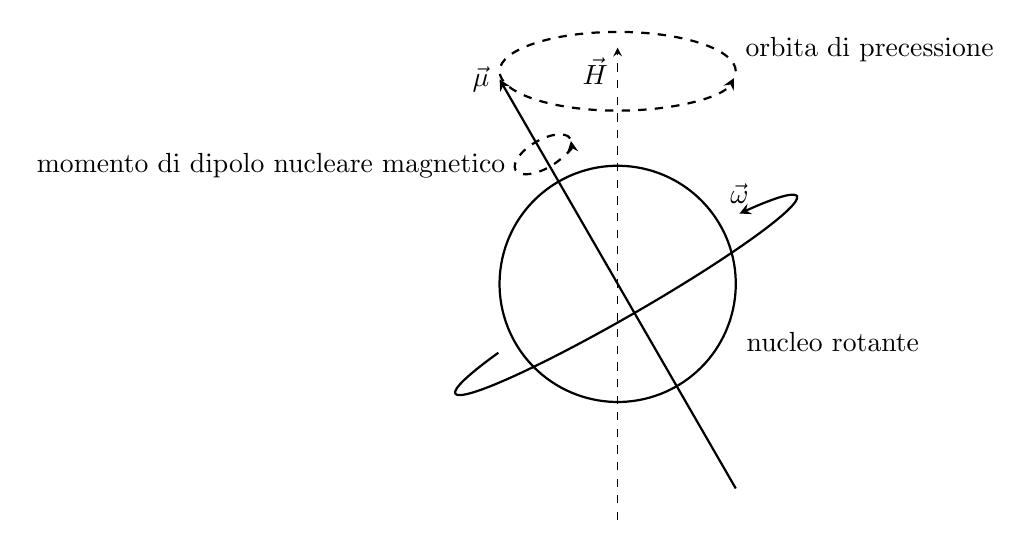
\begin{tikzpicture}[>=stealth]
% Linea tratteggiata NON ruotata
\draw[->, dashed] (0,-3)--(0,3) node[below left] {$\vec{H}$};; % al centro del cerchio
% Ellisse orientata in alto con centro sull'asse tratteggiato
\draw[dashed, thick, ->] (1.5,2.7) arc[start angle=0, end angle=350, x radius=1.5cm, y radius=0.5cm];
\node[above right] at (1.5,2.7) {orbita di precessione};

\node[right] at (-7.5,1.5) {momento di dipolo nucleare magnetico};

% Tutto il resto ruotato di 30°
\begin{scope}[rotate=30]
\shade[opacity=0] (0,0) circle(1.5); 
\draw[thick] (0,0) circle(1.5); 
\node at (2,-2) {nucleo rotante};

\draw[thick, ->] (0,-3)--(0,3) node[left] {$\vec{\mu}$};
\draw[->, dashed, thick] (0.4,1.9) arc[start angle=0, end angle=350, x radius=0.4cm, y radius=0.18cm];


\draw[thick, ->] (180:1.75) arc[start angle=135, end angle=405, x radius=2.5cm, y radius=0.25cm] node[above] {$\vec{\omega}$};
\end{scope}
\end{tikzpicture}
}
\caption{Moto di precessione del momento magnetico}
\label{fig:3_spin}
\end{figure}

Confrontando l'equazione ottenuta per il momento angolare:

\[
\dfrac{d\vec{L}}{dt} = \gamma\vec{L} \times \vec{B} = - \gamma\vec{B} \times \vec{L}
\]

Con la relazione generale che lega la rotazione di un vettore alla velocità angolare:

\[
d\vec{v} = \vec{\Omega} \times \vec{v}dt
\]

è evidente che la velocità angolare del moto di precessione è data da:

\[
\vec{\Omega} = - \gamma\vec{B}
\]

Con questa definizione, è possibile scrivere:

\[
\dfrac{d\vec{L}}{dt} = \vec{\Omega} \times \vec{L}
\]

Il modulo di questa velocità angolare è chiamato \textbf{Frequenza di Larmor} e rappresenta la frequenza angolare con cui il momento $\vec{\mu}$ precede attorno al campo $\vec{B}$:

\[
\omega_L = |\vec{\Omega}| = |\gamma| B
\]

\section{Diamagnetismo}\label{diamagnetismo}
I materiali diamagnetici sono caratterizzati da atomi che, se immersi in un campo magnetico $\vec{B}$, sviluppano un momento magnetico aggiuntivo ($\Delta \vec{\mu}$) che si \textbf{oppone} al campo applicato ($\vec{B}$). Il diamagnetismo è un fenomeno universale, presente in tutti i materiali, dovuto alla variazione del moto orbitale degli elettroni per effetto del campo esterno (Legge di Lenz).

Si suppone di applicare lentamente un campo magnetico a un atomo di materiale diamagnetico. Il suo nucleo, avendo una massa molto maggiore dell'elettrone può essere ritenuto fermo, mentre l'elettrone ruota interno al nucleo. Questo movimento può essere assimilato a una spira di raggio \(r\) percorsa da corrente centrata sul nucleo.

\begin{figure}[ht]
\centering
\resizebox{0.49\textwidth}{!}{%
\begin{tikzpicture}[>=Stealth, font=\sffamily]

% Orbita
\draw[thick] (0,0) circle (3cm);

% Protone al centro
\fill[blue!70!black] (0,0) circle (0.4cm);
\node[text=white, font=\bfseries] at (0,0) {+};
\node[below=6pt] at (0,-0.4) {Proton};

% Elettrone sul bordo sinistro
\fill[red!70!black] (-3,0) circle (0.25cm);
\node[text=white, font=\bfseries] at (-3,0) {-};
\node[above left=2pt] at (-3,0) {Electron};

% Freccia E (tangente alla circonferenza, verso il basso)
\draw[->, thick] (-3,-0.25) -- (-3,-1.2);
\node[left] at (-3,-1.2) {$E$};

% Freccia F_B (perpendicolare a E, verso il centro)
\draw[->, thick] (-2.75,0) -- (-1.90,0);
\node[above] at (-2,0) {$F_B$};

% Frecce di moto lungo l'orbita
\foreach \angle in {30,150,270} {
    \draw[->, thick] (\angle:3cm) arc[start angle=\angle,end angle=\angle+20,radius=3cm];
}

% Campo magnetico esterno (X simboli)
\foreach \x/\y in {-1.5/1.5,1.5/1.5,-1.5/-1.5,1.5/-1.5,0/2,0/-2} {
    \node at (\x,\y) {\Large $\times$};
}

% Etichetta External B
\node[right] at (1,1) {External B};

\end{tikzpicture}
}
\caption{Nucleo immerso in un campo magnetico}
\label{fig:3_AtomoMagnetic}
\end{figure}

Il campo magnetico \(\vec{B}\), variabile nel tempo e nello spazio, si concatena con la spira, provocando la generazione di una forza elettromagnetica data dalla legge di Faraday:

\[
\oint_{C}{\vec{E} \cdot d\vec{C}} = - \dfrac{\partial}{\partial t}\int_{S}{\vec{B} \cdot d\vec{S}}
\]

dove \(S\) è la superficie della spira e \(\partial S = C\) il suo contorno. Se il campo \(\vec{B}\) è costante sulla superficie della spira può essere portato fuori dal simbolo di integrale:

\[
\vec{E} \cdot \oint_{C}{d\vec{C}} = - \dfrac{\partial}{\partial t}\vec{B} \cdot \int_{S}{d\vec{S}}
\]

Ne discende che il campo elettrico è anch'esso uniforme sulla spira e parallelo, in ogni punto, a \(d\vec{C}\). Per una circonferenza risulta:

\[
E2\pi r = \pi r^{2}\left( - \dfrac{\partial B}{\partial t} \right)
\]

Dato che \(B\) è una funzione solo del tempo, la derivata parziale si riduce a una totale. Semplificando \(\pi r\) si ottiene:

\[
E = - \dfrac{r}{2}\dfrac{dB}{dt}
\]

Il campo elettrico produce un momento torcente sull'elettrone, dato dalla relazione:

\[
\vec{\tau} = q\vec{r} \times \vec{E}
\]

Dato che il campo elettrico è ortogonale al raggio, essendo ortogonale anche al campo magnetico \(\vec{B}\), il modulo del momento torcente, esplicitando anche la carica dell'elettrone, può essere espresso come:

\[
\tau = - erE
\]

Sostituendo il campo elettrico prima determinato, si ha:

\[
\tau = e\dfrac{r^{2}}{2}\dfrac{dB}{dt}
\]

Per la seconda legge di Newton \(dL\backslash dt = \tau\), si ottiene:

\[
\dfrac{dL}{dt} = e\dfrac{r^{2}}{2}\dfrac{dB}{dt}
\]

Si integra tra \(t_{0}\), tempo di applicazione del campo magnetico, e \(t_{1}\) tempo in cui il campo \(B\) raggiunge il suo valore massimo:

\[
\int_{t_{0}}^{t_{1}}{\dfrac{dL}{dt}dt} = e\dfrac{r^{2}}{2}\int_{t_{0}}^{t_{1}}{\dfrac{dB}{dt}dt}
\]

Risolvendo si ha:

\[
L\left( t_{1} \right) - L\left( t_{0} \right) = e\dfrac{r^{2}}{2}\left\lbrack B\left( t_{1} \right) - B\left( t_{0} \right) \right\rbrack
\]

Inizialmente il campo è nullo \(B\left( t_{0} \right) = 0\), per cui la differenza di momento angolare è data da:

\[
{\Delta}L = e\dfrac{r^{2}}{2}B
\]

dove \(B\) è il massimo valore del campo.

Il momento magnetico dell'elettrone intorno al nucleo è antiparallelo al momento angolare. Le due quantità sono legate dal rapporto giromagnetico:

\[
{\Delta}\mu = - \dfrac{e}{2m}{\Delta}L
\]

Sostituendo l'espressione della differenza del momento angolare, si ottiene:

\[
{\Delta}\mu = - \dfrac{e^{2}r^{2}}{4m}B
\]

In linea di principio l'orbita descritta dall'elettrone dovrebbe variare per l'applicazione del campo magnetico.

\begin{figure}[ht]
\centering
\resizebox{0.53\textwidth}{!}{%
\begin{tikzpicture}[>=Stealth, font=\sffamily]

% Nucleo
\fill[red!70!black] (0,0) circle (0.4cm);
\node[text=white, font=\bfseries] at (0,0) {+};
\node[below=4pt] at (0,-0.4) {Nucleo};

% Orbita
\draw[orange, thick, ->] (2,0) arc[start angle=0,end angle=360,radius=2cm];
\node at (2.6,-0.2) {Orbita};

% Elettrone
\fill[blue!70!black] (0,2) circle (0.25cm);
\node[text=white, font=\bfseries] at (0,2) {-};
\node[right=6pt] at (0.25,2) {Elettrone};

% Forza centrifuga
\draw[->, thick] (0,2.25) -- (0,3);
\node[above] at (0,3) {Forza centrifuga};

% Forza di attrazione elettrostatica (con allineamento corretto)
\draw[->, thick] (0,1.75) -- (0,1);
\node[align=center,left] at (-0.1,1.5) {Forza di attrazione\\elettrostatica};

\end{tikzpicture}
}
\caption{Elettrone in equilibrio sull'orbita}
\label{fig:3_EquiElettrone}
\end{figure}

Un elettrone orbitante è mantenuto, infatti, in equilibrio dalla forza centripeta (\(F_{c}\)) e dell'iterazione coulombiana con il nucleo (\(F_{e}\)):

\[
F_{e} = F_{c}
\]

Sostituendo le relative espressioni nell'ipotesi che il nucleo sia composto da un solo elettrone, si ha:

\[
m\dfrac{v^{2}}{r} = \dfrac{1}{4\pi\varepsilon_{0}}\dfrac{e^{2}}{r^{2}}
\]

La variazione di velocità indotta dal campo elettrico dopo l'introduzione del campo \(dB\) è data dalla forza che il campo esercita:

\[
F = \dfrac{dp}{dt} = m\dfrac{dv}{dt}
\]

La forza può essere espressa in termini di campo elettrico. Dalla definizione di campo elettrico, per l'elettrone risulta:

\[
E = \dfrac{F}{q} \Leftrightarrow F = - eE
\]

Dunque, la variazione di quantità di moto può essere espressa come:

\[
- eE = m\dfrac{dv}{dt}
\]

Il campo elettrico, per la legge di Faraday, è legato al campo magnetico dalla relazione:

\[
E = - \dfrac{r}{2}\dfrac{d\vec{B}}{dt}
\]

Ricavando:

\[
- eE = m\dfrac{dv}{dt} \Leftrightarrow e\dfrac{r}{2}\dfrac{d\vec{B}}{dt} = m\dfrac{dv}{dt}
\]

Si analizza la sola variazione di velocità subita dall'elettrone:

\[
dv = \dfrac{er}{2m}dB
\]

A causa della variazione di velocità, anche l'accelerazione centripeta \(\alpha\) varia. Ricorrendo allo sviluppo in serie di Taylor, trascurando gli ordini superiori al primo, si ha:

\[
\alpha + d\alpha = \dfrac{v^{2}}{r} + d\left( \dfrac{v^{2}}{r} \right) = \dfrac{v^{2}}{r} + \dfrac{2vdv}{r}\  + o\left( \dfrac{1}{r^{2}}dr \right) + o\left( dv^{2} \right)
\]

Dopo l'applicazione del campo magnetico, bisogna considerare anche la forza di Lorentz nel bilancio delle forze sull'elettrone. La forza di Lorentz e quella elettrostatica sono concordi, dunque, affinché l'elettrone sia in equilibrio, la velocità deve aumentare per incrementare la forza centripeta:

\[
\dfrac{mv^{2}}{r} + \dfrac{2mvdv}{r} = \dfrac{1}{4\pi\varepsilon_{0}}\dfrac{e^{2}}{r^{2}} + evdB
\]

Si è visto che:

\[
dv = \dfrac{er}{2m}dB
\]

Sostituendo nel bilancio, si ha:

\[
\dfrac{mv^{2}}{r} + \dfrac{2mv}{r}\dfrac{er}{2m}dB = \dfrac{1}{4\pi\varepsilon_{0}}\dfrac{e^{2}}{r^{2}} + evdB \Leftrightarrow \dfrac{mv^{2}}{r} + vedB = \dfrac{1}{4\pi\varepsilon_{0}}\dfrac{e^{2}}{r^{2}} + evdB
\]

Per cui si ottiene l'equazione dell'equilibrio prima dell'applicazione del campo esterno:

\[
\dfrac{mv^{2}}{r} = \dfrac{1}{4\pi\varepsilon_{0}}\dfrac{e^{2}}{r^{2}}
\]

Dopo l'applicazione del campo magnetico, l'equilibrio dell'elettrone è ottenuto mediante una sola variazione della velocità di rotazione. La variazione del raggio è influente per ordini superiori, dunque, in prima analisi, è perfettamente trascurabile. La cancellazione dei termini di ordine superiore ($\pm evdB$) dimostra che, se si ignora la variazione di raggio, la variazione di velocità indotta ($2mvdv/r$) è esattamente ciò che è richiesto dalla forza aggiuntiva di Lorentz ($evdB$) per mantenere l'equilibrio (cioè, $F_{centripeta} = F_{Lorentz} + F_{Coulomb}$).

Per i materiali diamagnetici la \textbf{permeabilità relativa} è circa unitaria, \(\mu_{r} \simeq 1\), con \textbf{valori leggermente inferiori all'unità} in modo da opporsi al campo applicato. Inoltre, essendo un fenomeno legato all'orbita elettronica, il diamagnetismo è presente in tutti i materiali.

\section{Paramagnetismo}\label{paramagnetismo}
A differenza del diamagnetismo (sempre presente in ogni materiale), il paramagnetismo è presente solamente nei materiali i cui atomi o molecole possiedono un \textbf{momento magnetico permanente} ($\vec{\mu} \neq 0$). Questo momento permanente è dovuto alla presenza di \textbf{elettroni spaiati} negli orbitali atomici, dove la cancellazione degli spin non è completa.

Per il principio di esclusione di Pauli, gli elettroni negli orbitali atomici si dispongono con spin antiparallelo, così da cancellare gli effetti degli spin stessi. Negli atomi in cui sono presenti elettroni spaiati, ovvero con orbitali atomici non completamente riempiti, la cancellazione degli spin non avviene, dunque, lo spin netto dell'atomo è diverso da zero. 

A livello macroscopico, gli spin dei vari costituenti del materiale si sommano, dando luogo alla magnetizzazione macroscopica. Quest'ultima è influenzata dalla presenza o meno di un campo magnetico.

In assenza di un campo magnetico esterno, il momento magnetico di ogni atomo è orientato in modo casuale a causa dell'agitazione termica, dunque, la magnetizzazione macroscopica media ($\vec{M}$) del materiale è nulla.

Applicato un campo magnetico esterno, invece, i singoli momenti magnetici (spin) subiscono un momento torcente che tende ad allinearli nella direzione del campo. Essi iniziano a precedere attorno alla direzione del campo con la frequenza di Larmor:

\[
\omega = \gamma B
\]

\begin{figure}[ht]
\centering
\resizebox{0.85\textwidth}{!}{%
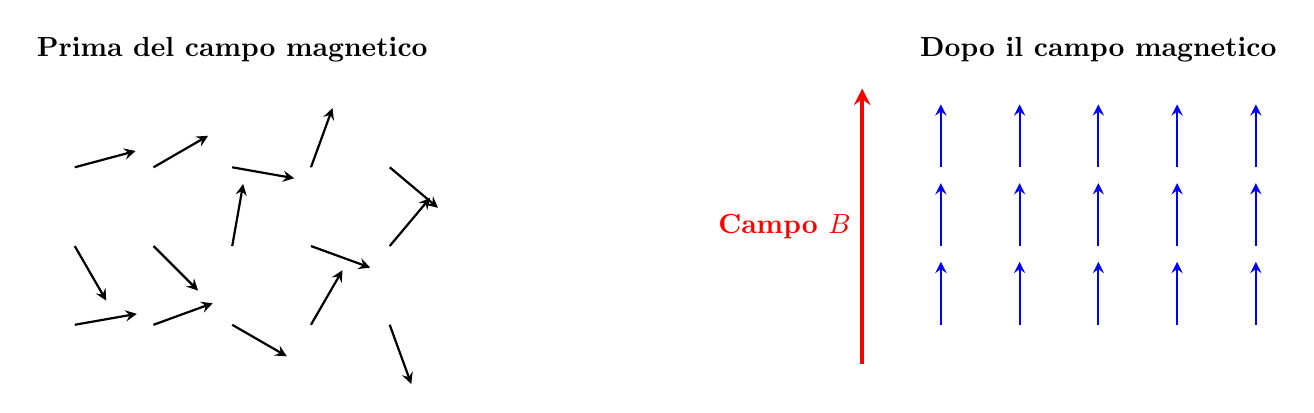
\begin{tikzpicture}[>=stealth, scale=1]

% Titoli
\node at (-8,3.5) {\textbf{Prima del campo magnetico}};
\node at (3,3.5) {\textbf{Dopo il campo magnetico}};

% Prima del campo magnetico (spin disordinati su griglia, molto a sinistra)
\foreach \x/\y/\angle in {-9/0/20, -8/0/-30, -7/0/60, -6/0/-70, -10/0/10,
                          -9/1/-45, -8/1/80, -7/1/-20, -6/1/50, -10/1/-60,
                          -9/2/30, -8/2/-10, -7/2/70, -6/2/-40, -10/2/15}
    \draw[->, thick] (\x,\y) -- ++({0.8*cos(\angle)},{0.8*sin(\angle)});

% Dopo il campo magnetico (spin allineati verso l'alto)
\foreach \x in {1,2,3,4,5}
  \foreach \y in {0,1,2}
    \draw[->, thick, blue] (\x,\y) -- ++(0,0.8);

% Campo magnetico indicato
\draw[->, ultra thick, red] (0,-0.5) -- (0,3) node[midway,left] {\textbf{Campo $B$}};

\end{tikzpicture}
}
\caption{Spin nei materiali paramagnetici}
\label{fig:3_ParaMagn}
\end{figure}

Il paramagnetismo è presente solo in alcune sostanze ed è un fenomeno debole. Esso è caratterizzato da una \textbf{suscettività magnetica} $\chi_m$ piccola e \textbf{positiva}:

\[
\chi_m > 0 \quad \text{e} \quad \chi_m \approx 10^{-3} - 10^{-5}
\]

Di conseguenza, la permeabilità magnetica relativa è lievemente maggiore dell'unità: $\mu_{r} = 1 + \chi_m \gtrsim 1$.


Si osservi che il vettore di magnetizzazione ($M$) è definito come la somma vettoriale dei momenti magnetici per unità di volume:

\[
\vec{M} = \dfrac{1}{V}\sum_{i}\vec{\mu}_i
\]

L'interazione del campo esterno con i momenti magnetici determina la magnetizzazione macroscopica $M$ del materiale, che in equilibrio termico è generalmente debole a causa del disorientamento termico.

La dipendenza della magnetizzazione dalla temperatura ($T$) è la firma distintiva del paramagnetismo, descritta dalla \textbf{Legge di Curie} (valida a basse induzioni e alte temperature):

\[
\chi_m = \dfrac{C}{T}
\]

Dove $C$ è la \textbf{Costante di Curie} del materiale. La suscettività è inversamente proporzionale alla temperatura: all'aumentare dell'agitazione termica, l'allineamento dei momenti magnetici diminuisce.

\section{Ferromagnetismo}
Il ferromagnetismo è la forma di magnetismo più intensa ed è caratteristica di materiali come ferro, cobalto, nichel e alcune loro leghe. A differenza del paramagnetismo, il ferromagnetismo non è causato solo dai momenti magnetici permanenti degli atomi, ma da una forte interazione di scambio quantistica tra gli spin degli elettroni degli atomi adiacenti. Questa interazione, molto più potente dell'agitazione termica, forza gli spin a orientarsi parallelamente su larga scala. Il risultato è la formazione di regioni microscopiche chiamate \textbf{domini di Weiss}, all'interno delle quali tutti i momenti magnetici sono perfettamente allineati, creando una magnetizzazione spontanea anche in assenza di un campo esterno ($\vec{B}_{est} = 0$). 

L'applicazione di un campo esterno debole fa crescere i domini favorevolmente orientati a spese di quelli sfavorevoli, portando a una magnetizzazione molto elevata. 

\begin{figure}[ht]
    \centering
    \resizebox{0.60\textwidth}{!}{%
    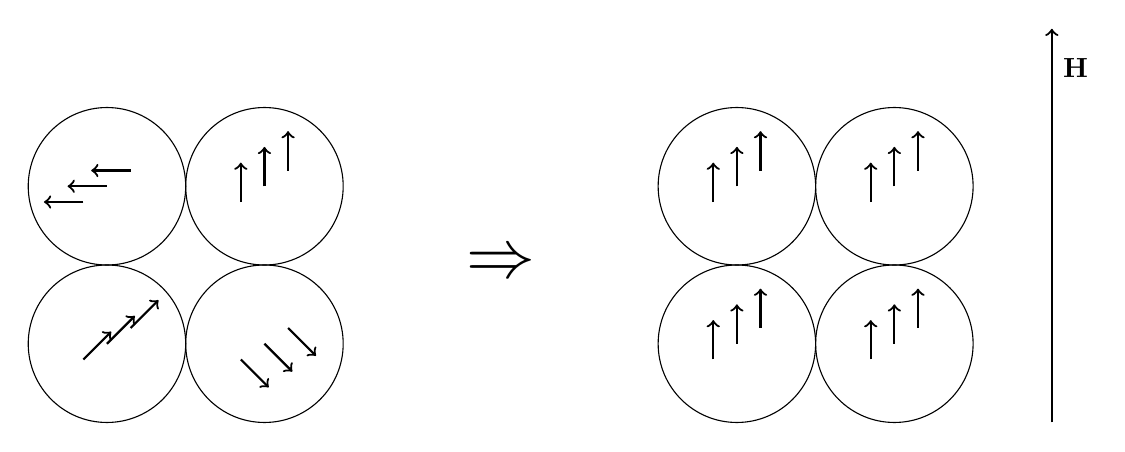
\begin{tikzpicture}[scale=1]

% --- Primo gruppo (sinistra) ---
\foreach \x/\y/\angle in {0/0/45, 2/0/-45, 0/2/180, 2/2/90} {
    \draw[rounded corners] (\x,\y) circle [x radius=1cm, y radius=1cm];
    % Più frecce parallele con variazione verticale e più corte
    \foreach \dx/\dy in {-0.3/-0.2, 0/0, 0.3/0.2} {
        \draw[->, thick] (\x+\dx,\y+\dy) -- ++({0.5*cos(\angle)},{0.5*sin(\angle)});
    }
}

% Freccia centrale
\node at (5,1) {\Huge $\Rightarrow$};

% --- Secondo gruppo (destra) ---
\foreach \x/\y in {8/0, 10/0, 8/2, 10/2} {
    \draw[rounded corners] (\x,\y) circle [x radius=1cm, y radius=1cm];
    % Più frecce parallele verso l'alto con variazione verticale e più corte
    \foreach \dx/\dy in {-0.3/-0.2, 0/0, 0.3/0.2} {
        \draw[->, thick] (\x+\dx,\y+\dy) -- ++(0,0.5);
    }
}

% Freccia H
\draw[->, thick] (12,-1) -- (12,4);
\node at (12.3,3.5) {\textbf{H}};

\end{tikzpicture}
    }
    \caption{Effetto dell'applicazione di un campo magnetico sui domini di Weiss}
    \label{fig:3_DomWeiss}
\end{figure}

I materiali ferromagnetici sono caratterizzati da una suscettività magnetica $\chi_m$ estremamente grande e positiva ($\chi_m \gg 10^5$) e una permeabilità magnetica relativa $\mu_r \gg 1$. 

Se la temperatura supera un valore critico chiamato temperatura di Curie ($T_C$), l'agitazione termica distrugge l'allineamento a lungo raggio, e il materiale perde il ferromagnetismo, diventando paramagnetico.

\begin{figure}[ht]
    \centering
    \resizebox{0.8\textwidth}{!}{%
    \begin{tikzpicture}[font=\sffamily]

% General styles
\tikzset{
  sample/.style={
    draw, thick,
    minimum width=6cm,
    minimum height=1.8cm,
    align=center,
    fill=#1!20
  },
  Bfield/.style={-Stealth, line width=0.9pt},
  mfield/.style={-Stealth, line width=0.8pt, red},
  domainline/.style={line width=0.9pt, blue, -Stealth},
  labeltop/.style={font=\large, yshift=3mm},
  labelbottom/.style={font=\footnotesize, yshift=-6mm, align=center}
}

%%%%%%%%%%%%%%%%%%%%%%%%%%%%
%% LAYOUT con due colonne
%%%%%%%%%%%%%%%%%%%%%%%%%%%%

\def\colsep{8cm}   % distanza tra colonne
\def\rowsep{6.5cm} % distanza tra righe


%%%%%%%%%%%%%%%%%%%%%%%%%%%%%%%%%%%%%%%%%%%%%%%%
%%%%%%%%%%%% 1) DIAMAGNETICO (colonna sinistra)
%%%%%%%%%%%%%%%%%%%%%%%%%%%%%%%%%%%%%%%%%%%%%%%%
\begin{scope}[xshift=-\colsep/2]

\node (dia) at (0,0) [sample=cyan] {};
\node[labeltop] at (dia.north) {\textbf{Diamagnetico}};
\node[labelbottom] at (dia.south)
{Momenti $m$ indotti opposti a $B$ \\ ($\chi < 0$)};

\foreach \y in {0.7,0.35,0,-0.35,-0.7}{
  \draw[Bfield] (-3,\y) -- (3,\y);
}

\foreach \x in {-1.5,-0.5,0.5,1.5}{
  \draw[mfield] (\x,0) -- ++(-0.5,0);
}

\begin{scope}[yshift=-3.5cm, scale=0.8]
  \draw[->] (0,0) -- (2,0) node[right]{\(B\)};
  \draw[->] (0,0) -- (0,1.2) node[above]{\(M\)};
  \draw[thick] (0.2,1.0) -- (1.8,0.3);
\end{scope}

\end{scope}


%%%%%%%%%%%%%%%%%%%%%%%%%%%%%%%%%%%%%%%%%%%%%%%%
%%%%%%%%%%%% 2) PARAMAGNETICO (colonna destra)
%%%%%%%%%%%%%%%%%%%%%%%%%%%%%%%%%%%%%%%%%%%%%%%%
\begin{scope}[xshift=\colsep/2]

\node (para) at (0,0) [sample=green] {};
\node[labeltop] at (para.north) {\textbf{Paramagnetico}};
\node[labelbottom] at (para.south)
{Momenti $m$ debolmente allineati a $B$ \\ ($\chi > 0$)};

\foreach \y in {0.7,0.35,0,-0.35,-0.7}{
  \draw[Bfield] (-3,\y) -- (3,\y);
}

\foreach \x in {-1.5,-0.5,0.5,1.5}{
  \draw[mfield] (\x,0) -- ++(0.5,0);
}

\begin{scope}[yshift=-3.5cm, scale=0.8]
  \draw[->] (0,0) -- (2,0) node[right]{\(B\)};
  \draw[->] (0,0) -- (0,1.2) node[above]{\(M\)};
  \draw[thick] (0.2,0.2) -- (1.8,1.0);
\end{scope}

\end{scope}


%%%%%%%%%%%%%%%%%%%%%%%%%%%%%%%%%%%%%%%%%%%%%%%%
%%%%%%% 3) FERROMAGNETICO (riga sotto, centrato)
%%%%%%%%%%%%%%%%%%%%%%%%%%%%%%%%%%%%%%%%%%%%%%%%
\begin{scope}[yshift=-\rowsep]

\node (ferro) at (0,0) [sample=orange] {};
\node[labeltop] at (ferro.north) {\textbf{Ferromagnetico}};
\node[labelbottom] at (ferro.south)
{Domini magnetici allineati; remanenza e isteresi};

\foreach \y in {0.7,0.35,0,-0.35,-0.7}{
  \draw[Bfield] (-3,\y) -- (3,\y);
}

\foreach \x in {-1.5,-0.5,0.5,1.5}{
  \draw[domainline] (\x,0) -- ++(0.5,0);
}

\foreach \x in {-1.0,-0.5,0,0.5}{
  \draw[dashed] (\x,-1) -- ++(0,2);
}

\begin{scope}[yshift=-3.5cm, scale=0.8]
  \draw[->] (-1.5,0) -- (1.5,0) node[right]{\(B\)};
  \draw[->] (0,-1.2) -- (0,1.4) node[above]{\(M\)};
  \draw[thick, rounded corners=3pt]
    (-1.1,-0.45) .. controls (-0.4,-0.9) and (0.4,-0.9) .. (1.1,-0.45)
    .. controls (0.45,0) and (0.5,0.6) .. (1.1,0.95)
    .. controls (0,1.2) and (-0,1.2) .. (-1.1,0.95)
    .. controls (-0.5,0.6) and (-0.5,0) .. (-1.1,-0.45);
\end{scope}

\end{scope}

\end{tikzpicture}
    }
    \caption{Risposta al campo magnetico da parte dei diversi materiali}
    \label{fig:3_DiffMaterial}
\end{figure}
